\documentclass[UTF8,a4paper,zihao=-4,fontset=windows]{ctexart}
\usepackage[margin=2.5cm]{geometry}
\usepackage{amsmath,amssymb,graphicx,booktabs,array,adjustbox,caption,float,needspace,longtable}
\usepackage[unicode,hidelinks]{hyperref}
\usepackage{fancyhdr}
\usepackage{tikz}
\usetikzlibrary{arrows.meta,positioning}
\setmainfont{Times New Roman}
\setlength{\parindent}{2em}
\linespread{1.16}
\setlength{\parskip}{0pt}
\setlength{\abovedisplayskip}{7pt}
\setlength{\belowdisplayskip}{7pt}
\setlength{\textfloatsep}{9pt}
\setlength{\intextsep}{9pt}
\captionsetup{font=small,labelfont=bf,textfont=bf,labelsep=space,justification=centering,singlelinecheck=false}
\captionsetup[table]{position=bottom,skip=5pt}
\captionsetup[figure]{position=bottom,skip=5pt}
\newcommand{\figtabnote}[1]{\par\vspace{3pt}{\fontsize{9}{11}\selectfont\raggedright\noindent 注：#1\par}}
\ctexset{section={format=\Large\heiti,beforeskip=12pt,afterskip=6pt},subsection={format=\large\heiti,beforeskip=9pt,afterskip=5pt}}
\pagestyle{fancy}\fancyhf{}\fancyfoot[C]{\thepage}\renewcommand{\headrulewidth}{0pt}
\setlength{\headheight}{14pt}
\setcounter{secnumdepth}{0}
\emergencystretch=2em
\begin{document}

\begin{center}{\zihao{2}\heiti 基于残差场景与滚动调整的微网购电及储能调控策略}\end{center}
\begin{center}\large\bfseries 摘\quad 要\end{center}
针对光伏出力、负载及电价变化下的微网购电问题，考虑日前预测难以覆盖日内偏差，建立由确定性线性规划、残差场景随机规划和日内滚动调整组成的调控模型。在满足逐时供电与储能约束的基础上，区分计划购电、计划调整和紧急购电三类费用，并以实际运行轨迹评价策略。
\par
针对问题一，将一天划分为144个10分钟时段，以储能侧充放电量为变量，建立含日初日末储电量相等约束的线性规划。求得全天购电量59482.70 kWh，费用35101.57元；储电量在1200—10800 kWh内变化。容量与功率的121组组合试验表明，所考察范围内费用为35056.72—40319.54元。
\par
针对问题二，采用最近同类型日预测负载、最近五日预测光伏，以最近十日配对残差构建场景，形成共同日前计划及场景补救决策。实际运行采用受储电量和功率约束的充放电规则。在2月1日至12月31日的334天内，总费用为1370.17万元，紧急购电量为12.79万kWh。
\par
针对问题三，按历史误差组合外部光伏预报与历史预测，在6、12、18时更新剩余时段购电计划。完整追索式方案费用为1326.66万元，较问题二降低3.18\%，紧急购电量减少83.46\%。消融试验中，仅在12、18时调整的方案费用最低，为1315.58万元，但紧急购电量较主方案增加，说明更新频次应结合费用和应急需求选择。
\par
针对问题四，利用历史同类型日电价和当日已观测电价预测未来价格，以实际电价结算。日前方案与滚动方案费用分别为1440.18万元和1395.35万元，后者节约3.11\%。保持日均电价的波动试验中，滚动方案节约率由1.17\%增至4.76\%。实际轨迹满足电量平衡、储电边界和跨日连续约束；结论适用于所给数据及所采用的储能计量约定。
\par
\textbf{关键词：}微网调控；残差场景；两阶段随机规划；滚动优化；储能调度
\par
\clearpage
\section{1 问题重述与分析}
\subsection{1.1 研究任务}
微网通过光伏、储能和外网购电共同满足小区负载。储能可以将低价时段的电量转移至高价时段，也可吸收暂时过剩的光伏电量，但其容量、功率和能量损耗限制了转移能力。问题的关键是提前购买多少电、何时调整承诺，以及预测偏差出现后如何调度储能。
\par
问题一给出固定电价、负载和一天的光伏预测，要求在0时确定全天计划，且日末储电量回到日初水平。问题二引入实际负载和光伏变化，普通购电按计划量付费，供电不足须以五倍现货电价紧急购电。问题三增加每日四次光伏预报，允许付费调整原计划，需判断额外预报是否值得使用。问题四进一步考虑实时电价波动，重新计算日前方案和滚动方案。各问均需给出题面指定日期、时段的购电与储能结果。
\par
\subsection{1.2 方法选择与研究思路}
微网与主电网的经济协调属于能量管理层问题，区别于电压、频率等快速控制问题[1]。题目未提供线路阻抗或节点结构，因此本文以10分钟电量平衡建模，不引入无法识别参数的交流潮流方程。
\par
问题一的费用和储能动态均为线性关系，采用线性规划可直接处理144个时段的耦合，无需引入启发式搜索。问题二的计划先于实际负载和光伏实现，具有“先承诺、后补救”的决策顺序，适合两阶段随机规划[2]。相较只使用一条预测曲线，历史残差场景能让计划同时考虑多个偏差路径；相较以所有最坏情况为目标的稳健模型，场景平均费用与本题的购电费用目标更直接对应。但有限历史场景不能保证覆盖未来所有偏差。
\par
问题三采用滚动优化：新信息到达后重新求解未来部分，已经执行的部分保持不变。该思路已有微网能量管理研究支持[3]。本文只调整购电与储能，不增加机组启停等整数决策。预测与权重选择均按时间先后进行，仅使用决策时刻以前的信息，遵循时间序列预测的滚动评价原则[4]。问题四保持原有供电模型，只扩展价格预测及结算，便于比较新增价格信息的作用。
\par
全文求解采用SciPy线性规划接口[5]和HiGHS求解器。稀疏线性规划及修正单纯形方法已有成熟算法研究[6]。文献支持方法选择，具体历史窗口、预测修正系数和终端价值均来自本题既有模型设置，不视为文献给出的通用最优参数。
\par
\begin{table}[H]\centering
\fontsize{9.5}{12}\selectfont\setlength{\tabcolsep}{4pt}\renewcommand{\arraystretch}{1.12}
\begin{adjustbox}{max width=\linewidth}\begin{tabular}{lccc}\toprule
\textbf{问题} & \textbf{新增条件} & \textbf{模型} & \textbf{评价依据}\\\midrule
一 & 供需曲线给定、日末闭合 & 确定性线性规划 & 日费用与可行性\\
二 & 实际负载和光伏未知 & 残差场景日前规划 & 实际费用与紧急购电\\
三 & 四次光伏预报及调整收费 & 追索式计划与滚动调整 & 费用、应急量及消融\\
四 & 未来实际电价未知 & 因果价格预测与滚动优化 & 信息对照及波动试验\\
\bottomrule\end{tabular}\end{adjustbox}
\caption{四问的决策条件与模型对应关系}
\end{table}
\begin{figure}[H]\centering
\begin{tikzpicture}[box/.style={draw,rounded corners=2pt,text width=3.35cm,minimum height=1.0cm,align=center,font=\small},>=Stealth]
\node[box] (a) at (0,0) {问题一\\确定性线性规划};
\node[box] (b) at (4,0) {问题二\\残差场景日前规划};
\node[box] (c) at (8,0) {问题三\\预报组合与滚动调整};
\node[box] (d) at (12,0) {问题四\\因果价格预测};
\draw[->] (a)--(b);\draw[->] (b)--(c);\draw[->] (c)--(d);
\node[draw,rounded corners=2pt,align=center,text width=11.6cm,font=\small] (e) at (8,-1.55) {历史信息生成预测与场景\quad{}→\quad{}因果执行\quad{}→\quad{}按实际电价结算};
\draw[->] (b.south)--(4,-.9)--(e.north -| b.south);
\draw[->] (c.south)--(e.north);
\draw[->] (d.south)--(12,-.9)--(e.north -| d.south);
\end{tikzpicture}
\caption{四问的模型递进与共同评价流程}
\figtabnote{历史信息生成预测与场景，实际运行后再计算费用。}
\end{figure}
\section{2 数据整理与建模假设}
\subsection{2.1 数据来源和时间对齐}
附件1提供144个时段的电价、负载与光伏预测功率；附件2提供2025年365天的实际负载和光伏功率；附件3每天有0、6、12、18时四次预报，每次包含未来24个整点的光伏功率；附件4给出365天的实际电价。数值区域检查未发现缺失或负值，因此未对原始功率与价格做异常值删除或平滑处理。附件3的合并日期单元格按同日四次预报补齐日期标签，保留其数值不变。
\par
设一天共有$N=144$个时段，时段$t=0,\ldots,143$对应区间$[t\Delta,(t+1)\Delta)$，其中$\Delta=1/6$小时。源表的00:10是第一个时段的右端点，24:00是最后一个时段的右端点。计算时按原顺序对应区间，不将功率序列平移一格。因此题面10:00—10:10的购电量取数组下标60。功率统一转换为时段电量：
\par
\begin{equation}
L_{i,t}=P^L_{i,t}\Delta,\qquad G_{i,t}=P^G_{i,t}\Delta. \tag{1}
\end{equation}
仿真从1月1日以6000 kWh开始连续运行，1月份用于形成历史预测与运行状态；按结果模板要求，费用及策略比较统计2月1日至12月31日，共334天。下文“统计期”均指这334天。2月1日的储电量继承1月31日运行结果，并不重置为6000 kWh。
\par
\subsection{2.2 建模假设及适用范围}
（1）将微网作为单节点能量系统，忽略线路损耗、通信时延和电压约束；储能损耗由效率参数计入。题目未给出这些附加参数，本文只讨论能量与费用调控。
\par
（2）充电效率和放电效率分别取0.9，即一次完整充放电的能量效率为0.81。储能不考虑自放电、寿命衰减和随荷电状态变化的效率，5000 kW功率上限在每个10分钟时段内恒定。
\par
（3）微网不向外网售电；超过负载且无法存储的电量计为余电。该限制是本模型的购电型运行假设，题面未规定售电价格。问题二至四允许紧急购电补足缺口，未额外设置外网供电容量上限，因此模型保障供电不等于证明现实外网不存在供电风险。
\par
（4）历史负载采用两类日：周五、周六为低负载类型，其他日期为另一类型。这是对附件中负载模式的经验分组，不将其解释为法定工作日、休息日划分。用近期样本代表短期未来，不借用待预测日的实际整日数据。
\par
（5）问题三以0时原计划为调整结算基准，减购部分保留原价的50\%作为违约费用；增购部分按原价的1.5倍支付。多次修订只结算各时段最终执行的版本，避免把同一时段反复修改的差额重复收费。问题四另外假设未来实际电价在决策时未知，预测电价用于优化，实际电价用于结算。
\par
（6）储能充放电的计量侧保留各问原模型定义。问题一的变量表示储能内部电量增减，5000 kW上限作用于储能侧；问题二至四的变量表示微网侧电量，上限作用于微网侧。二者换算后对应的微网侧功率边界不同，不能直接比较其充放电极值，也不能据此宣称四问采用完全相同的物理功率边界。问题一的结论以储能侧上限解释为前提，相关换算见第4节。
\par
\section{3 符号说明与公共约束}
\begin{table}[H]\centering
\fontsize{9.5}{12}\selectfont\setlength{\tabcolsep}{4pt}\renewcommand{\arraystretch}{1.12}
\begin{adjustbox}{max width=\linewidth}\begin{tabular}{lcc}\toprule
\textbf{符号} & \textbf{含义} & \textbf{单位}\\\midrule
$i,t,k$ & 日期、时段及场景下标 & —\\
$N,\Delta,K$ & 日时段数、时长及场景数：144、1/6、10 & —、h、—\\
$P^L,P^G$ & 负载功率、光伏功率 & kW\\
$L,G$ & 时段负载电量、光伏电量 & kWh\\
$g^0,g^{\tau},g^{\mathrm{fin}}$ & 原计划、更新计划、最终计划购电量 & kWh\\
$c,d$ & 问题二至四的微网侧充电量、放电量 & kWh\\
$\bar c,\bar d$ & 问题一的储能侧充电量、放电量 & kWh\\
$S$ & 储能设备内部存储电量 & kWh\\
$e,z$ & 紧急购电量、未使用余电量 & kWh\\
$r,x$ & 相对原计划的减购量、增购量 & kWh\\
$\pi,\widehat\pi$ & 实际交易电价、预测电价 & 元/kWh\\
$\eta,E_{\max}$ & 单向效率0.9、时段能量上限833.3333 & —、kWh\\
$v,\epsilon$ & 终端储电价值0.42、吞吐引导系数0.001 & 元/kWh\\
\bottomrule\end{tabular}\end{adjustbox}
\caption{主要符号与单位}
\end{table}
表中功率用于预测，电量用于优化与结算。日期下标$i$在单日模型中省略；上标$k$表示场景，上标0表示0时原计划，上标$\tau$表示在时段$\tau$开始时作出的更新。预测量用帽号表示。
\par
对问题二至四，功率上限对应时段电量上限$E_{\max}=5000\Delta=833.3333$ kWh。实际调度满足
\par
\begin{equation}
g_t+G_t+d_t+e_t=L_t+c_t+z_t,\qquad S_{t+1}=S_t+\eta c_t-d_t/\eta, \tag{2}
\end{equation}
\begin{equation}
1200\le S_t\le10800,\quad 0\le c_t,d_t\le E_{\max},\quad g_t,e_t,z_t\ge0. \tag{3}
\end{equation}
其中$z_t$可包含光伏富余和按计划购买但无法使用的电量，不能全部解释为弃光。式（2）写成等式是因为将富余量单列为$z_t$，并未把题面“供电不可低于负载”加强为不许出现富余电量。
\par
规划模型使用较窄的未来储电范围$1500\le S_t^k\le10500$，两端各保留300 kWh安全裕度；日初实测状态仍服从物理范围1200—10800 kWh。实际运行允许使用该裕度。问题二至四不施加每日首末储电量相等约束，而以$S_{i+1,0}=S_{i,144}$连接相邻日期。
\par
\section{4 问题一：确定性日前购电模型}
\subsection{4.1 线性规划的建立与求解}
对给定负载和光伏预测，决定每个时段购电量$g_t$以及储能侧充、放电量$\bar c_t,\bar d_t$，使全天费用最小：
\par
\begin{equation}
\min C_1=\sum_{t=0}^{143}\pi_tg_t. \tag{4}
\end{equation}
储能侧充入$\bar c_t$需要微网提供$\bar c_t/\eta$，储能侧放出$\bar d_t$只能向微网供给$\eta\bar d_t$，故有
\par
\begin{equation}
g_t+G_t+\eta\bar d_t=L_t+\bar c_t/\eta,\qquad S_{t+1}=S_t+\bar c_t-\bar d_t. \tag{5}
\end{equation}
\begin{equation}
\begin{gathered}
0\le\bar c_t,\bar d_t\le833.3333,\qquad g_t\ge0,\\
1200\le S_t\le10800,\qquad S_0=S_{144}=6000.
\end{gathered} \tag{6}
\end{equation}
该模型在问题一给定曲线上不额外设置余电变量，求得的解满足式（5）。由于变量连续，目标和约束均线性，共有577个变量、290个等式约束。调用SciPy的linprog并选择HiGHS，结果状态为最优。因此全局最优结论限于式（4）—（6）定义的线性规划；它不是问题二至四因果控制策略的全局最优证明。
\par
若改用微网侧变量，则$c_t=\bar c_t/\eta$、$d_t=\eta\bar d_t$，相应上限分别为925.9259和750.0000 kWh，即5555.56和4500.00 kW。换算时必须同步换算边界。本文保留储能侧数值，以免只替换公式便改变原问题一计算结果的物理含义。
\par
\subsection{4.2 购电计划与储能运行}
\begin{table}[H]\centering
\fontsize{9.5}{12}\selectfont\setlength{\tabcolsep}{4pt}\renewcommand{\arraystretch}{1.12}
\begin{adjustbox}{max width=\linewidth}\begin{tabular}{lccccc}\toprule
\textbf{时间段} & \shortstack{\textbf{购电量}\\{\normalfont （kWh）}} & \textbf{时间段} & \shortstack{\textbf{购电量}\\{\normalfont （kWh）}} & \textbf{时间段} & \shortstack{\textbf{购电量}\\{\normalfont （kWh）}}\\\midrule
10:00-10:10 & 0.00 & 12:00-12:10 & 573.01 & 14:00-14:10 & 0.00\\
16:00-16:10 & 445.43 & 18:00-18:10 & 531.89 & 20:00-20:10 & 0.00\\
全天购电量 & 59482.70 & 全天购电费/元 & 35101.57 & 计量单位 & kWh、元\\
\bottomrule\end{tabular}\end{adjustbox}
\caption{问题一指定时段购电量及全天费用}
\end{table}
\begin{table}[H]\centering
\fontsize{9.5}{12}\selectfont\setlength{\tabcolsep}{4pt}\renewcommand{\arraystretch}{1.12}
\begin{adjustbox}{max width=\linewidth}\begin{tabular}{lccccc}\toprule
\textbf{时间段} & \textbf{充电量} & \textbf{放电量} & \textbf{时间段} & \textbf{充电量} & \textbf{放电量}\\\midrule
0:00-4:00 & 3966.67 & 0.00 & 4:00-8:00 & 833.33 & 7073.16\\
8:00-12:00 & 3975.83 & 1892.22 & 12:00-16:00 & 5090.76 & 101.22\\
16:00-20:00 & 0.00 & 6422.37 & 20:00-24:00 & 4800.00 & 3177.63\\
0:00储电量 & 6000.00 & — & 24:00储电量 & 6000.00 & —\\
\bottomrule\end{tabular}\end{adjustbox}
\caption{问题一储能侧充放电及首末储电量（kWh）}
\end{table}
图2给出供需条件、充放电时段和储电量轨迹。储能先吸收低价电量和光伏富余，在较高电价及负载缺口出现时放电；日末再恢复到6000 kWh。全天储能侧累计充电、放电量均为18666.60 kWh。部分四小时窗口中充、放电累计量均为正，是窗口内不同时段切换造成的，并不表示同一10分钟时段同时充放电。逐时检查的同时充放电时段数为0。
\par
\begin{figure}[H]\centering
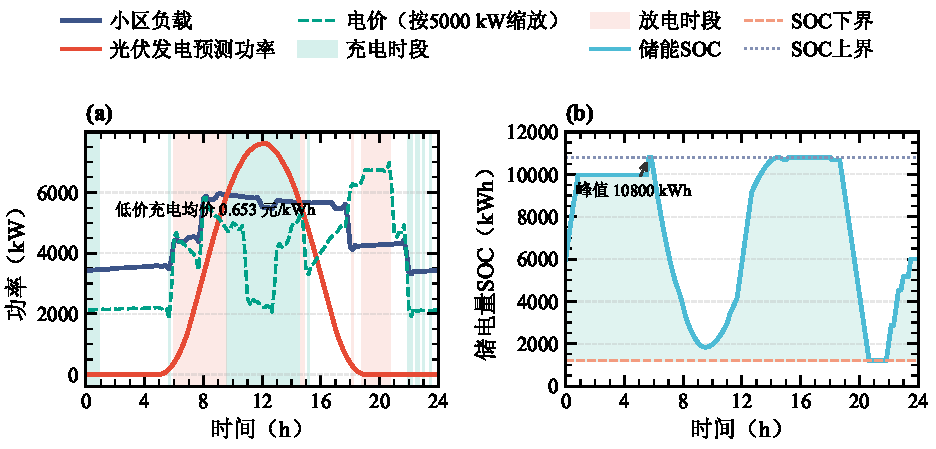
\includegraphics[width=.92\linewidth,height=7.0cm,keepaspectratio]{../new_figures_main/Q1_F1_optimal_dispatch.pdf}
\caption{问题一供需曲线与储能调控轨迹}
\figtabnote{左图将电价乘5000后与功率曲线同轴展示，背景区分充、放电时段；右图为储电量及其边界。}
\end{figure}
\subsection{4.3 容量与功率灵敏度}
以6000 kWh为中心，将可用储电区间写成$[6000-4800a,6000+4800a]$，其中$a=0.50,0.55,\ldots,1.00$；将储能侧时段功率上限乘以系数$b$，取值为0.40、0.48、0.56、0.64、0.72、0.80、0.88、0.96、1.00、1.10、1.20。逐组求解得到121组费用。这里$a$缩放的是可用储电窗口，不能将$a=0.5$简单说成额定容量降至6000 kWh。
\par
\begin{table}[H]\centering
\fontsize{9.5}{12}\selectfont\setlength{\tabcolsep}{4pt}\renewcommand{\arraystretch}{1.12}
\begin{adjustbox}{max width=\linewidth}\begin{tabular}{lccc}\toprule
\textbf{功率系数} & \textbf{容量系数0.50} & \textbf{容量系数0.75} & \textbf{容量系数1.00}\\\midrule
0.40 & 40319.54 & 38385.22 & 37665.34\\
0.80 & 40044.58 & 37210.27 & 35327.90\\
1.00 & 40011.01 & 37155.98 & 35101.57\\
1.20 & 39993.29 & 37131.03 & 35056.72\\
\bottomrule\end{tabular}\end{adjustbox}
\caption{容量窗口与储能侧功率系数的费用节选（元）}
\end{table}
在选定网格内，增加容量窗口和功率上限不会缩小可行域，因此最小费用不应上升，这与计算结果一致。网格最低费用为35056.72元，相比原参数仅减少44.84元，说明在容量窗口保持最大值时，继续增加所考察的功率上限带来的节约有限。该试验未计入设备扩容成本，不能据此确定经济最优设备规格；也未进行效率参数扫描，不能推导效率灵敏度结论。
\par
\section{5 问题二：残差场景下的日前购电与实际调度}
\subsection{5.1 点预测和配对残差场景}
负载预测取最近三个同类型日的均值，光伏预测取最近五日均值，分别记为$\widehat P^L_{i,t}$和$\widehat P^G_{i,t}$。历史不足时使用当时已经可获得的样本；1月运行只用于预热，不计入统计期。对每个过去日期$h$，用当日当时可生成的预测计算残差，不以事后重新拟合的结果替换历史预测。
\par
从最近十个历史日期取配对的负载与光伏残差，形成$K=10$个等权场景：
\par
\begin{equation}
\begin{aligned}
L^k_{i,t}&=\Delta\,[\widehat P^L_{i,t}+\varepsilon^L_{h_k,t}]_+,\\
G^k_{i,t}&=\Delta\,[\widehat P^G_{i,t}+\varepsilon^G_{h_k,t}]_+,
\end{aligned}\qquad [x]_+=\max(x,0). \tag{7}
\end{equation}
同一场景的两类残差来自同一个历史日，从而保留该日负载与光伏误差的共同变化；保留全天残差路径也保留了样本内的时序形态。非负截断只作用于生成的预测或场景，不改动原始观测。这里没有假设残差服从正态分布，也没有随机抽取大量蒙特卡洛样本。
\par
\begin{figure}[H]\centering
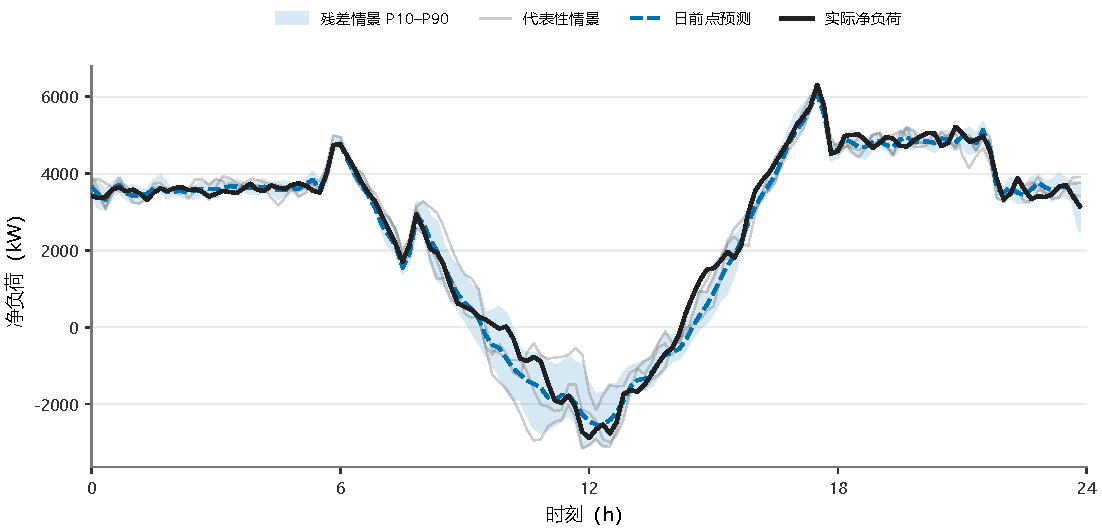
\includegraphics[width=.92\linewidth,height=7.0cm,keepaspectratio]{../new_figures_main/Q2_F2_uncertainty_scenarios.pdf}
\caption{典型日净负荷场景与实际轨迹}
\figtabnote{P10—P90为十条历史残差场景的经验分位带，不是经校准的概率置信区间。}
\end{figure}
\subsection{5.2 两阶段随机线性规划}
第一阶段确定所有场景共用的购电计划$g_t$；第二阶段分别安排场景下的充放电、紧急购电和余电。以场景平均运行代价评价第一阶段计划：
\par
\begin{equation}
\min\;\sum_t\pi_tg_t+\frac1K\sum_{k=1}^K\left[5\sum_t\pi_te_t^k+\epsilon\sum_t(c_t^k+d_t^k)-vS_{144}^k\right]. \tag{8}
\end{equation}
约束为各场景的式（2）、式（3）及未来规划储电范围1500—10500 kWh，其中$\epsilon=0.001$元/kWh，$v=0.42$元/kWh。微小吞吐惩罚用于抑制没有经济价值的循环，终端储电价值用于减轻日末过度放电的短视倾向。二者是优化引导项，不计入实际向外网支付的购电费，也不应称为电池真实折旧费用。
\par
采用场景路径的第二阶段决策相当于假定在该阶段知晓完整场景，而真实运行时未来仍不可知。因此式（8）是两阶段近似，并非具有完整非预见性约束的多阶段随机控制。本文用下一小节的因果运行轨迹检验其实际表现，不直接把规划场景中的紧急购电量作为最终结果。
\par
\subsection{5.3 因果运行规则与结算}
每个时段先接收实际负载和光伏，计算计划购电后的净缺口$R_t=L_t-G_t-g_t$。若$R_t\ge0$，优先用可用储能补足，剩余部分紧急购买：
\par
\begin{equation}
d_t=\min\{R_t,E_{\max},\eta(S_t-1200)\},\quad e_t=R_t-d_t,\quad c_t=z_t=0. \tag{9}
\end{equation}
若$R_t<0$，先在功率和容量范围内充电，其余计为余电：
\par
\begin{equation}
c_t=\min\{-R_t,E_{\max},(10800-S_t)/\eta\},\quad z_t=-R_t-c_t,\quad d_t=e_t=0. \tag{10}
\end{equation}
更新$S_{t+1}$后进入下一时段。该规则按缺口符号选择充电或放电，从执行机制上避免同一时段同时充放电。日末状态传入下一日。实际费用为
\par
\begin{equation}
C_2=\sum_{i,t}\pi_tg_{i,t}+5\sum_{i,t}\pi_te_{i,t}. \tag{11}
\end{equation}
普通购电按计划量收费，计划电量即使转为余电，也不从第一项扣除。模型通过较高的紧急购电代价与过量计划的支出之间的权衡，形成购电承诺。
\par
\subsection{5.4 统计期结果与典型日结果}
\begin{table}[H]\centering
\fontsize{9.5}{12}\selectfont\setlength{\tabcolsep}{4pt}\renewcommand{\arraystretch}{1.12}
\begin{adjustbox}{max width=\linewidth}\begin{tabular}{lc}\toprule
\textbf{指标} & \textbf{数值}\\\midrule
统计天数/d & 334\\
计划购电费/元 & 12925565.04\\
调整费/元 & 0.00\\
紧急购电费/元 & 776093.47\\
总费用/元 & 13701658.50\\
0时计划购电量/kWh & 20632061.35\\
最终计划购电量/kWh & 20632061.35\\
紧急购电量/kWh & 127912.33\\
发生紧急购电天数/d & 107\\
余电量/kWh & 1674121.12\\
\bottomrule\end{tabular}\end{adjustbox}
\caption{问题二统计期实际结果}
\end{table}
负载预测MAE为137.31 kW，RMSE为189.83 kW；光伏预测MAE为151.52 kW，RMSE为304.47 kW。光伏RMSE明显大于MAE，说明少数较大偏差对平方误差的影响更强。因此仅报告平均费用不足以反映运行风险，还需查看紧急购电量及发生日期。统计期有107天发生紧急购电，说明300 kWh规划裕度和十条残差场景没有完全覆盖实际偏差。
\par
\begin{figure}[H]\centering
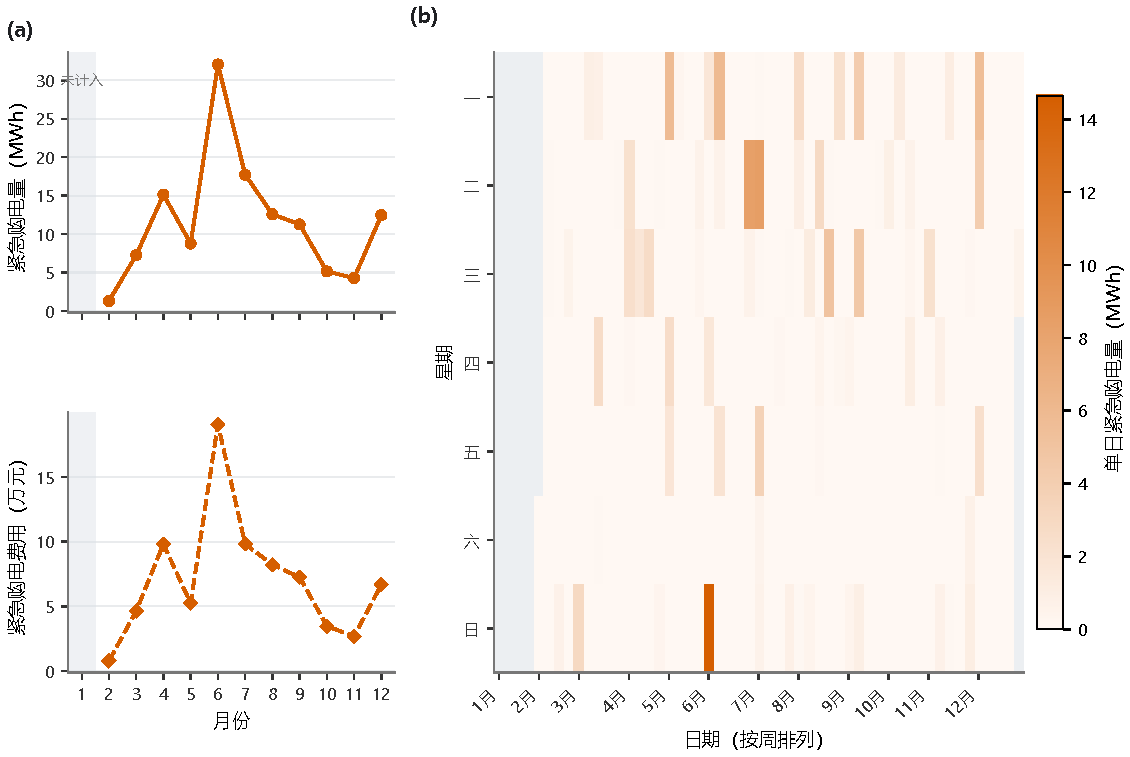
\includegraphics[width=.92\linewidth,height=8.8cm,keepaspectratio]{../new_figures_main/Q2_F3_annual_risk_profile.pdf}
\caption{问题二费用组成与紧急购电分布}
\figtabnote{月份汇总和逐日记录均取实际执行结果。}
\end{figure}
以下各表沿用题面表1、表2的排列：指定时段为10分钟购电量，储能按四小时窗口累计；费用为包含紧急购电的当日总费用。储能量均按微网侧计量。
\par
\begin{table}[H]\centering
\fontsize{9.5}{12}\selectfont\setlength{\tabcolsep}{4pt}\renewcommand{\arraystretch}{1.12}
\begin{adjustbox}{max width=\linewidth}\begin{tabular}{lccccc}\toprule
\textbf{时间段} & \shortstack{\textbf{购电量}\\{\normalfont （kWh）}} & \textbf{时间段} & \shortstack{\textbf{购电量}\\{\normalfont （kWh）}} & \textbf{时间段} & \shortstack{\textbf{购电量}\\{\normalfont （kWh）}}\\\midrule
10:00–10:10 & 0.00 & 12:00–12:10 & 625.40 & 14:00–14:10 & 0.00\\
16:00–16:10 & 455.28 & 18:00–18:10 & 671.19 & 20:00–20:10 & 0.00\\
全天购电量 & 66148.82 & 全天总费用/元 & 40940.02 & 单位 & kWh、元\\
\bottomrule\end{tabular}\end{adjustbox}
\caption{问题二 2025-03-20 指定时段购电量与全天费用}
\end{table}
\begin{table}[H]\centering
\fontsize{9.5}{12}\selectfont\setlength{\tabcolsep}{4pt}\renewcommand{\arraystretch}{1.12}
\begin{adjustbox}{max width=\linewidth}\begin{tabular}{lccccc}\toprule
\textbf{时间段} & \textbf{充电量} & \textbf{放电量} & \textbf{时间段} & \textbf{充电量} & \textbf{放电量}\\\midrule
00:00–04:00 & 7146.43 & 164.49 & 04:00–08:00 & 2130.64 & 4704.60\\
08:00–12:00 & 5033.40 & 2777.38 & 12:00–16:00 & 4620.42 & 501.13\\
16:00–20:00 & 34.33 & 5509.90 & 20:00–24:00 & 681.65 & 2906.81\\
0:00储电量 & 2541.29 & — & 24:00储电量 & 1818.69 & —\\
\bottomrule\end{tabular}\end{adjustbox}
\caption{问题二 2025-03-20 储能充放电量及首末储电量（kWh）}
\end{table}
\begin{table}[H]\centering
\fontsize{9.5}{12}\selectfont\setlength{\tabcolsep}{4pt}\renewcommand{\arraystretch}{1.12}
\begin{adjustbox}{max width=\linewidth}\begin{tabular}{lccccc}\toprule
\textbf{时间段} & \shortstack{\textbf{购电量}\\{\normalfont （kWh）}} & \textbf{时间段} & \shortstack{\textbf{购电量}\\{\normalfont （kWh）}} & \textbf{时间段} & \shortstack{\textbf{购电量}\\{\normalfont （kWh）}}\\\midrule
10:00–10:10 & 0.00 & 12:00–12:10 & 0.00 & 14:00–14:10 & 0.00\\
16:00–16:10 & 179.07 & 18:00–18:10 & 193.13 & 20:00–20:10 & 0.00\\
全天购电量 & 33335.65 & 全天总费用/元 & 19637.89 & 单位 & kWh、元\\
\bottomrule\end{tabular}\end{adjustbox}
\caption{问题二 2025-06-21 指定时段购电量与全天费用}
\end{table}
\begin{table}[H]\centering
\fontsize{9.5}{12}\selectfont\setlength{\tabcolsep}{4pt}\renewcommand{\arraystretch}{1.12}
\begin{adjustbox}{max width=\linewidth}\begin{tabular}{lccccc}\toprule
\textbf{时间段} & \textbf{充电量} & \textbf{放电量} & \textbf{时间段} & \textbf{充电量} & \textbf{放电量}\\\midrule
00:00–04:00 & 425.71 & 415.84 & 04:00–08:00 & 1182.56 & 1843.75\\
08:00–12:00 & 10168.34 & 0.00 & 12:00–16:00 & 0.00 & 0.00\\
16:00–20:00 & 33.10 & 5057.02 & 20:00–24:00 & 751.22 & 2595.70\\
0:00储电量 & 2711.70 & — & 24:00储电量 & 3002.87 & —\\
\bottomrule\end{tabular}\end{adjustbox}
\caption{问题二 2025-06-21 储能充放电量及首末储电量（kWh）}
\end{table}
\begin{table}[H]\centering
\fontsize{9.5}{12}\selectfont\setlength{\tabcolsep}{4pt}\renewcommand{\arraystretch}{1.12}
\begin{adjustbox}{max width=\linewidth}\begin{tabular}{lccccc}\toprule
\textbf{时间段} & \shortstack{\textbf{购电量}\\{\normalfont （kWh）}} & \textbf{时间段} & \shortstack{\textbf{购电量}\\{\normalfont （kWh）}} & \textbf{时间段} & \shortstack{\textbf{购电量}\\{\normalfont （kWh）}}\\\midrule
10:00–10:10 & 0.00 & 12:00–12:10 & 439.89 & 14:00–14:10 & 0.00\\
16:00–16:10 & 527.13 & 18:00–18:10 & 752.85 & 20:00–20:10 & 3.63\\
全天购电量 & 66611.15 & 全天总费用/元 & 43062.88 & 单位 & kWh、元\\
\bottomrule\end{tabular}\end{adjustbox}
\caption{问题二 2025-09-23 指定时段购电量与全天费用}
\end{table}
\begin{table}[H]\centering
\fontsize{9.5}{12}\selectfont\setlength{\tabcolsep}{4pt}\renewcommand{\arraystretch}{1.12}
\begin{adjustbox}{max width=\linewidth}\begin{tabular}{lccccc}\toprule
\textbf{时间段} & \textbf{充电量} & \textbf{放电量} & \textbf{时间段} & \textbf{充电量} & \textbf{放电量}\\\midrule
00:00–04:00 & 7572.93 & 17.01 & 04:00–08:00 & 1976.79 & 4704.25\\
08:00–12:00 & 4078.03 & 1896.62 & 12:00–16:00 & 4448.31 & 660.67\\
16:00–20:00 & 24.02 & 5699.28 & 20:00–24:00 & 498.69 & 2583.15\\
0:00储电量 & 2107.46 & — & 24:00储电量 & 1556.39 & —\\
\bottomrule\end{tabular}\end{adjustbox}
\caption{问题二 2025-09-23 储能充放电量及首末储电量（kWh）}
\end{table}
\begin{table}[H]\centering
\fontsize{9.5}{12}\selectfont\setlength{\tabcolsep}{4pt}\renewcommand{\arraystretch}{1.12}
\begin{adjustbox}{max width=\linewidth}\begin{tabular}{lccccc}\toprule
\textbf{时间段} & \shortstack{\textbf{购电量}\\{\normalfont （kWh）}} & \textbf{时间段} & \shortstack{\textbf{购电量}\\{\normalfont （kWh）}} & \textbf{时间段} & \shortstack{\textbf{购电量}\\{\normalfont （kWh）}}\\\midrule
10:00–10:10 & 0.00 & 12:00–12:10 & 856.43 & 14:00–14:10 & 0.00\\
16:00–16:10 & 813.89 & 18:00–18:10 & 678.35 & 20:00–20:10 & 0.00\\
全天购电量 & 94191.33 & 全天总费用/元 & 61188.39 & 单位 & kWh、元\\
\bottomrule\end{tabular}\end{adjustbox}
\caption{问题二 2025-12-21 指定时段购电量与全天费用}
\end{table}
\begin{table}[H]\centering
\fontsize{9.5}{12}\selectfont\setlength{\tabcolsep}{4pt}\renewcommand{\arraystretch}{1.12}
\begin{adjustbox}{max width=\linewidth}\begin{tabular}{lccccc}\toprule
\textbf{时间段} & \textbf{充电量} & \textbf{放电量} & \textbf{时间段} & \textbf{充电量} & \textbf{放电量}\\\midrule
00:00–04:00 & 8110.27 & 183.59 & 04:00–08:00 & 2652.95 & 1604.01\\
08:00–12:00 & 5355.11 & 6619.39 & 12:00–16:00 & 7222.51 & 2433.99\\
16:00–20:00 & 56.39 & 5377.06 & 20:00–24:00 & 386.15 & 2962.32\\
0:00储电量 & 1823.00 & — & 24:00储电量 & 1916.51 & —\\
\bottomrule\end{tabular}\end{adjustbox}
\caption{问题二 2025-12-21 储能充放电量及首末储电量（kWh）}
\end{table}
\begin{table}[H]\centering
\fontsize{9.5}{12}\selectfont\setlength{\tabcolsep}{4pt}\renewcommand{\arraystretch}{1.12}
\begin{adjustbox}{max width=\linewidth}\begin{tabular}{lccccccc}\toprule
\multicolumn{2}{c}{\textbf{03-20}} & \multicolumn{2}{c}{\textbf{06-21}} & \multicolumn{2}{c}{\textbf{09-23}} & \multicolumn{2}{c}{\textbf{12-21}}\\
\cmidrule(lr){1-2} \cmidrule(lr){3-4} \cmidrule(lr){5-6} \cmidrule(lr){7-8}
\textbf{时段} & \shortstack{\textbf{购电量}\\{\normalfont （kWh）}} & \textbf{时段} & \shortstack{\textbf{购电量}\\{\normalfont （kWh）}} & \textbf{时段} & \shortstack{\textbf{购电量}\\{\normalfont （kWh）}} & \textbf{时段} & \shortstack{\textbf{购电量}\\{\normalfont （kWh）}}\\\midrule
无 & 0.00 & 无 & 0.00 & 21:00–21:10 & 11.80 & 无 & 0.00\\
— & — & — & — & 21:20–21:40 & 53.83 & — & —\\
合计 & 0.00 & 合计 & 0.00 & 合计 & 65.63 & 合计 & 0.00\\
\bottomrule\end{tabular}\end{adjustbox}
\caption{问题二四个典型日紧急购电（kWh）}
\end{table}
四个典型日中，3月20日和6月21日无需紧急购电，9月23日发生65.63 kWh紧急购电。典型日结果用于展示时段安排，全年表现仍以334天完整统计为依据，不能用少数日期替代整体评价。
\par
\section{6 问题三：预报组合与日内滚动调整}
\subsection{6.1 预报对齐、组合及当日修正}
附件3的整点预报先线性插值到10分钟右端点网格。0时发布时以0作为边界锚点；6、12、18时发布时，以该时刻之前最后一个已完成时段的光伏观测为边界锚点，再连接至发布后第一个整点预报。仅提取当日剩余时段，未将次日部分纳入跨午夜的优化。
\par
设$A_{i,t}^{\tau}$为附件3插值预报，$H_{i,t}$为历史均值预测。按最近30天同一发布时间、同一剩余时域的MAE选择组合权重：
\par
\begin{equation}
w_i^{\tau}\in\arg\min_{w\in\{0,0.1,\ldots,1\}}\frac{1}{|\mathcal H_i|(144-\tau)}\sum_{h\in\mathcal H_i}\sum_{t=\tau}^{143}\left|wA_{h,t}^{\tau}+(1-w)H_{h,t}-P^G_{h,t}\right|. \tag{12}
\end{equation}
由此得到$\widehat P_{i,t}^{G,\tau}=w_i^{\tau}A_{i,t}^{\tau}+(1-w_i^{\tau})H_{i,t}$。集合$\mathcal H_i$只含日期$i$以前的样本，权重不使用当前日剩余时段的真实光伏。
\par
日内负载修正利用当日已观测误差。设其均值为$b$、最近一个误差为$u$，对距更新时刻第$\ell$个时段的预测采用
\par
\begin{equation}
\widehat P_{t}^{L,\tau}=\left[\widehat P_t^{L,0}+b+0.65^{\ell}(u-b)\right]_+. \tag{13}
\end{equation}
光伏修正取更新前最近一个0时组合预测大于1 kW的时段$a$，以$\kappa=P^G_a/\widehat P_a^{G,0}$表示实际出力相对原预测的比例；不存在该时段时令$\kappa=1$。按距离衰减该比例偏差：
\par
\begin{equation}
\widetilde P_t^{G,\tau}=\left[\widehat P_t^{G,\tau}\{1+(\kappa-1)0.94^{\ell}\}\right]_+. \tag{14}
\end{equation}
式（14）是经验比例修正。代码中使用“晴空指数”名称，但其分母是日前组合预测，并非由太阳辐射物理模型计算的晴空功率。本文据此将它称为光伏比例修正，避免赋予其未建立的物理含义。发布时间对应的历史残差按更新后的预测重新形成场景。
\par
\subsection{6.2 原计划、调整变量与结算模型}
将0时计划记为$g_t^0$。对每条场景设置减购量$r_t^k$和增购量$x_t^k$，6时以前二者固定为0，6时及以后允许追索，且$0\le r_t^k\le g_t^0$。在0时提前考虑未来可能调整的代价：
\par
\begin{equation}
\begin{aligned}
\min\;&\sum_t\pi_tg_t^0+\frac1K\sum_k\Big[\sum_t\pi_t(-0.5r_t^k+1.5x_t^k+5e_t^k)\\
&\hspace{32mm}+\epsilon\sum_t(c_t^k+d_t^k)-vS_{144}^k\Big].
\end{aligned} \tag{15}
\end{equation}
各场景电量平衡中的计划电量相应替换为$g_t^0-r_t^k+x_t^k$。式（15）的场景减购、增购代表提前评估的补救机会，实际执行的调整仍须在信息发布后重新求解。
\par
在$\tau=36,72,108$，以当前实际储电量为初值，更新负载、光伏及残差场景，对剩余时段使用共同调整决策：
\par
\begin{equation}
g_t^{\tau}=g_t^0-r_t^{\tau}+x_t^{\tau},\qquad0\le r_t^{\tau}\le g_t^0,\quad x_t^{\tau}\ge0,\quad t\ge\tau. \tag{16}
\end{equation}
优化目标为剩余调整费用与平均场景应急、吞吐和终端代价之和，约束与问题二相同。0时已承诺费用在此时是常数，不影响最优调整量，故从该次优化目标中省略。重要的是，式（16）始终相对0时原计划，而不是相对上一轮修订量。
\par
最终计划按实际适用时段拼接：0—6时用$g^0$，6—12时用$g^{36}$，12—18时用$g^{72}$，18—24时用$g^{108}$。记拼接结果为$g^{\mathrm{fin}}$，则总费用为
\par
\begin{equation}
\begin{aligned}
C_3&=C_{\mathrm{plan}}+C_{\mathrm{adj}}+C_{\mathrm{em}},\\
C_{\mathrm{plan}}&=\sum_{i,t}\pi_tg_{i,t}^0,\\
C_{\mathrm{adj}}&=\sum_{i,t}\pi_t\left[-0.5(g_{i,t}^0-g_{i,t}^{\mathrm{fin}})_++1.5(g_{i,t}^{\mathrm{fin}}-g_{i,t}^0)_+\right],\\
C_{\mathrm{em}}&=5\sum_{i,t}\pi_te_{i,t}.
\end{aligned} \tag{17}
\end{equation}
例如原计划100 kWh、最终80 kWh，计划费100倍单价加上调整项负10倍单价，合计为80 kWh正常购电费加20 kWh的50\%违约费。这样既保留减购部分的违约成本，也避免在原计划已全额计费后再重复加收该部分的50\%。
\par
\begin{figure}[H]\centering
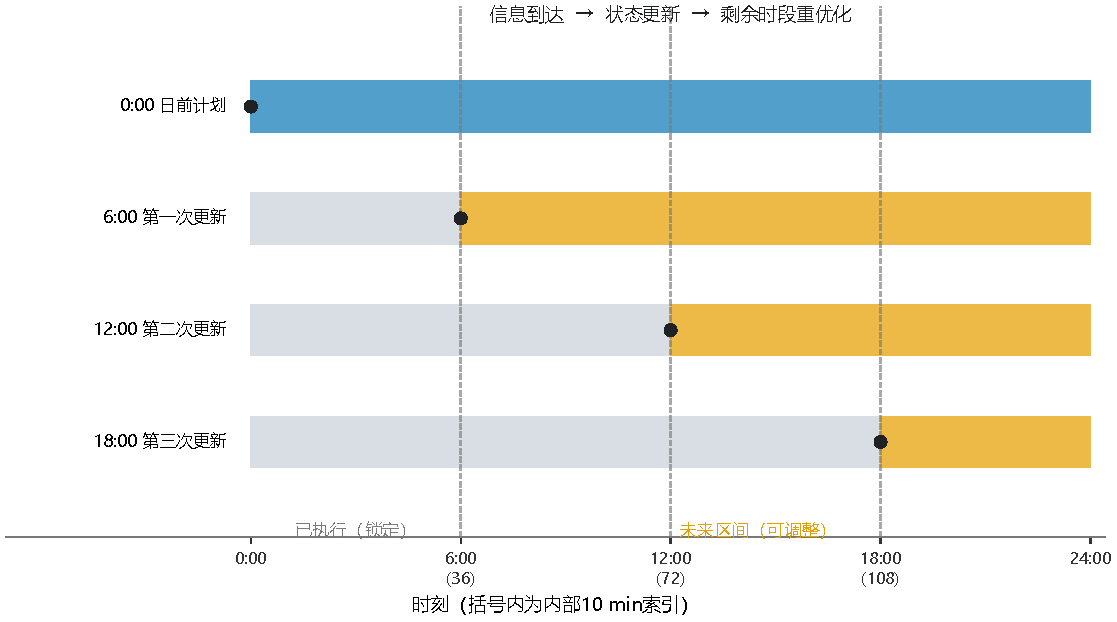
\includegraphics[width=.92\linewidth,height=6.8cm,keepaspectratio]{../new_figures_main/Q3_F1_rolling_timeline.pdf}
\caption{问题三日内滚动调整流程}
\figtabnote{0时制定原计划，6、12、18时用新预报和实测储电量优化当日剩余时段；每段采用最近一次可用计划。}
\end{figure}
\subsection{6.3 预报效果与运行费用}
\begin{table}[H]\centering
\fontsize{9.5}{12}\selectfont\setlength{\tabcolsep}{4pt}\renewcommand{\arraystretch}{1.12}
\begin{adjustbox}{max width=\linewidth}\begin{tabular}{lcccc}\toprule
\textbf{发布时间} & \textbf{附件3} & \textbf{历史预测} & \textbf{组合预测} & \textbf{组合后比例修正}\\\midrule
0:00 & 197.49 & 151.52 & 129.67 & 129.67\\
6:00 & 158.52 & 200.90 & 136.26 & 196.90\\
12:00 & 75.25 & 145.79 & 74.32 & 97.79\\
18:00 & 10.02 & 2.15 & 2.01 & 1.85\\
\bottomrule\end{tabular}\end{adjustbox}
\caption{各发布时间光伏预测MAE（kW）}
\figtabnote{按该次发布剩余时段评价。}
\end{table}
组合预测在四个发布时间的MAE均低于直接使用附件3；但加入比例修正后，6时MAE从136.26升至196.90 kW，12时从74.32升至97.79 kW。可见近期实际与原预测的比例不一定能代表未来天气，修正可能放大偏差。18时修正后的误差较小，也受到剩余时段以夜间低出力为主的影响，不能直接推断该方法在相同预测长度下优于上午。
\par
\begin{table}[H]\centering
\fontsize{9.5}{12}\selectfont\setlength{\tabcolsep}{4pt}\renewcommand{\arraystretch}{1.12}
\begin{adjustbox}{max width=\linewidth}\begin{tabular}{lcc}\toprule
\textbf{指标} & \textbf{问题二} & \textbf{问题三}\\\midrule
统计天数/d & 334 & 334\\
计划购电费/元 & 12925565.04 & 12408349.81\\
调整费/元 & 0.00 & 753729.66\\
紧急购电费/元 & 776093.47 & 104543.26\\
总费用/元 & 13701658.50 & 13266622.73\\
0时计划购电量/kWh & 20632061.35 & 20060179.42\\
最终计划购电量/kWh & 20632061.35 & 20518906.35\\
紧急购电量/kWh & 127912.33 & 21152.53\\
发生紧急购电天数/d & 107 & 87\\
余电量/kWh & 1674121.12 & 1424175.34\\
\bottomrule\end{tabular}\end{adjustbox}
\caption{问题二与问题三主方案的统计期比较}
\end{table}
主方案统计期总费用为13266622.73元，比问题二减少435035.77元；紧急购电量由127912.33降至21152.53 kWh，降幅83.46\%。费用由计划费12408349.81元、调整费753729.66元和紧急购电费104543.26元组成。调整需要付费，但整体策略降低的计划及应急支出超过了调整费用。
\par
主方案同时改变了光伏预测、日前追索结构和日内调整方式，因此相对问题二的节约是整个策略的收益，不能全部归因于某一个发布时间或某一种预测修正。日费用也不保证逐日下降：四个指定日期的主方案总费用均高于问题二，说明统计期收益由其他日期的改善共同形成。
\par
\subsection{6.4 额外发布时间的必要性}
\begin{table}[H]\centering
\fontsize{9.5}{12}\selectfont\setlength{\tabcolsep}{4pt}\renewcommand{\arraystretch}{1.12}
\begin{adjustbox}{max width=\linewidth}\begin{tabular}{lccc}\toprule
\textbf{方案} & \shortstack{\textbf{总费用}\\{\normalfont （万元）}} & \shortstack{\textbf{紧急购电量}\\{\normalfont （kWh）}} & \textbf{日前追索}\\\midrule
完整追索式计划 & 1326.66 & 21152.53 & 是\\
仅0:00，不调整 & 1353.90 & 110241.21 & 否\\
仅6:00 & 1358.61 & 56310.78 & 否\\
仅12:00 & 1321.49 & 42052.27 & 否\\
仅18:00 & 1321.34 & 33058.91 & 否\\
6:00+12:00 & 1335.62 & 26449.71 & 否\\
12:00+18:00 & 1315.58 & 33029.76 & 否\\
6:00+12:00+18:00（无追索） & 1330.14 & 17970.87 & 否\\
问题2方案 & 1370.17 & 127912.33 & —\\
完美信息基准 & 1225.48 & 0.00 & —\\
\bottomrule\end{tabular}\end{adjustbox}
\caption{更新时点和日前追索的方案比较}
\end{table}
在已计算的方案中，只用6时更新的费用高于不更新，说明增加一次预报并不自动产生净收益。仅12时或仅18时更新的方案都降低了费用；12时与18时联合调整的费用最低，为13155783.13元。因而若仅以本组试验的统计期总费用选择，可优先使用12、18时更新，不必把所有发布时间一律加入。
\par
本文保留完整追索式计划作为主方案，以对应每日三个时点均可修订的运行流程。它比12、18时方案多支出110839.60元，但紧急购电量减少11877.23 kWh。这个比较同时改变了更新时点和0时的追索结构，不能把全部差异解释为6时更新的边际作用。固定三个更新时点后，加入日前追索使费用由13301412.48降至13266622.73元，但紧急购电量从17970.87增至21152.53 kWh；因此追索也并非在所有指标上占优。
\par
这里仅比较已经计算的有限方案，未包含6时与18时组合，也未搜索任意更新时间。12、18时方案是所测方案中的费用最小者，不是所有可能控制策略的全局最优方案。供给完全已知的计算结果称为“完美信息基准”；其使用逐日优化和终端价值，未构造与整个统计期实际结算目标完全一致的全局问题，故不将其称为严格下界。
\par
\subsection{6.5 典型日完整结果}
以下购电表中的每个时段先列0时原计划，再列最终执行计划，记为“原/终”。全天购电量同样给出两种数量；全天费用按式（17）计算。储能表为最终实际运行结果，单位均为kWh。
\par
\begin{table}[H]\centering
\fontsize{9.5}{12}\selectfont\setlength{\tabcolsep}{4pt}\renewcommand{\arraystretch}{1.12}
\begin{adjustbox}{max width=\linewidth}\begin{tabular}{lccccc}\toprule
\textbf{时间段} & \shortstack{\textbf{购电量}\\{\normalfont （kWh）}} & \textbf{时间段} & \shortstack{\textbf{购电量}\\{\normalfont （kWh）}} & \textbf{时间段} & \shortstack{\textbf{购电量}\\{\normalfont （kWh）}}\\\midrule
10:00–10:10 & 0.00 / 0.00 & 12:00–12:10 & 538.09 / 618.49 & 14:00–14:10 & 0.00 / 0.00\\
16:00–16:10 & 538.26 / 538.26 & 18:00–18:10 & 671.19 / 679.70 & 20:00–20:10 & 0.00 / 0.00\\
全天购电量 & 65024.60 / 65917.49 & 全天总费用/元 & 44142.02 & 单位 & kWh、元\\
\bottomrule\end{tabular}\end{adjustbox}
\caption{问题三 2025-03-20 指定时段购电量与全天费用（原计划/最终计划）}
\end{table}
\begin{table}[H]\centering
\fontsize{9.5}{12}\selectfont\setlength{\tabcolsep}{4pt}\renewcommand{\arraystretch}{1.12}
\begin{adjustbox}{max width=\linewidth}\begin{tabular}{lccccc}\toprule
\textbf{时间段} & \textbf{充电量} & \textbf{放电量} & \textbf{时间段} & \textbf{充电量} & \textbf{放电量}\\\midrule
00:00–04:00 & 7394.59 & 14.97 & 04:00–08:00 & 1829.31 & 5691.28\\
08:00–12:00 & 2935.78 & 2506.79 & 12:00–16:00 & 7072.08 & 255.20\\
16:00–20:00 & 153.57 & 5259.70 & 20:00–24:00 & 681.04 & 2717.52\\
0:00储电量 & 2024.09 & — & 24:00储电量 & 1811.09 & —\\
\bottomrule\end{tabular}\end{adjustbox}
\caption{问题三 2025-03-20 储能充放电量及首末储电量（kWh）}
\end{table}
\begin{table}[H]\centering
\fontsize{9.5}{12}\selectfont\setlength{\tabcolsep}{4pt}\renewcommand{\arraystretch}{1.12}
\begin{adjustbox}{max width=\linewidth}\begin{tabular}{lccccc}\toprule
\textbf{时间段} & \shortstack{\textbf{购电量}\\{\normalfont （kWh）}} & \textbf{时间段} & \shortstack{\textbf{购电量}\\{\normalfont （kWh）}} & \textbf{时间段} & \shortstack{\textbf{购电量}\\{\normalfont （kWh）}}\\\midrule
10:00–10:10 & 0.00 / 0.00 & 12:00–12:10 & 0.00 / 0.00 & 14:00–14:10 & 0.00 / 0.00\\
16:00–16:10 & 128.77 / 128.77 & 18:00–18:10 & 0.00 / 0.00 & 20:00–20:10 & 0.00 / 0.00\\
全天购电量 & 32788.93 / 33321.63 & 全天总费用/元 & 19727.57 & 单位 & kWh、元\\
\bottomrule\end{tabular}\end{adjustbox}
\caption{问题三 2025-06-21 指定时段购电量与全天费用（原计划/最终计划）}
\end{table}
\begin{table}[H]\centering
\fontsize{9.5}{12}\selectfont\setlength{\tabcolsep}{4pt}\renewcommand{\arraystretch}{1.12}
\begin{adjustbox}{max width=\linewidth}\begin{tabular}{lccccc}\toprule
\textbf{时间段} & \textbf{充电量} & \textbf{放电量} & \textbf{时间段} & \textbf{充电量} & \textbf{放电量}\\\midrule
00:00–04:00 & 198.67 & 306.84 & 04:00–08:00 & 1389.78 & 1440.01\\
08:00–12:00 & 9670.60 & 0.00 & 12:00–16:00 & 0.00 & 0.00\\
16:00–20:00 & 41.50 & 5273.24 & 20:00–24:00 & 686.38 & 2623.75\\
0:00储电量 & 2607.81 & — & 24:00储电量 & 2680.65 & —\\
\bottomrule\end{tabular}\end{adjustbox}
\caption{问题三 2025-06-21 储能充放电量及首末储电量（kWh）}
\end{table}
\begin{table}[H]\centering
\fontsize{9.5}{12}\selectfont\setlength{\tabcolsep}{4pt}\renewcommand{\arraystretch}{1.12}
\begin{adjustbox}{max width=\linewidth}\begin{tabular}{lccccc}\toprule
\textbf{时间段} & \shortstack{\textbf{购电量}\\{\normalfont （kWh）}} & \textbf{时间段} & \shortstack{\textbf{购电量}\\{\normalfont （kWh）}} & \textbf{时间段} & \shortstack{\textbf{购电量}\\{\normalfont （kWh）}}\\\midrule
10:00–10:10 & 0.00 / 0.00 & 12:00–12:10 & 386.56 / 0.00 & 14:00–14:10 & 0.00 / 0.00\\
16:00–16:10 & 573.36 / 573.36 & 18:00–18:10 & 752.85 / 765.47 & 20:00–20:10 & 3.63 / 7.30\\
全天购电量 & 64801.74 / 68391.05 & 全天总费用/元 & 46234.62 & 单位 & kWh、元\\
\bottomrule\end{tabular}\end{adjustbox}
\caption{问题三 2025-09-23 指定时段购电量与全天费用（原计划/最终计划）}
\end{table}
\begin{table}[H]\centering
\fontsize{9.5}{12}\selectfont\setlength{\tabcolsep}{4pt}\renewcommand{\arraystretch}{1.12}
\begin{adjustbox}{max width=\linewidth}\begin{tabular}{lccccc}\toprule
\textbf{时间段} & \textbf{充电量} & \textbf{放电量} & \textbf{时间段} & \textbf{充电量} & \textbf{放电量}\\\midrule
00:00–04:00 & 7513.62 & 5.55 & 04:00–08:00 & 3016.80 & 3965.15\\
08:00–12:00 & 5253.03 & 1896.62 & 12:00–16:00 & 1333.90 & 425.56\\
16:00–20:00 & 107.98 & 5807.95 & 20:00–24:00 & 479.75 & 2638.16\\
0:00储电量 & 2100.88 & — & 24:00储电量 & 1658.82 & —\\
\bottomrule\end{tabular}\end{adjustbox}
\caption{问题三 2025-09-23 储能充放电量及首末储电量（kWh）}
\end{table}
\begin{table}[H]\centering
\fontsize{9.5}{12}\selectfont\setlength{\tabcolsep}{4pt}\renewcommand{\arraystretch}{1.12}
\begin{adjustbox}{max width=\linewidth}\begin{tabular}{lccccc}\toprule
\textbf{时间段} & \shortstack{\textbf{购电量}\\{\normalfont （kWh）}} & \textbf{时间段} & \shortstack{\textbf{购电量}\\{\normalfont （kWh）}} & \textbf{时间段} & \shortstack{\textbf{购电量}\\{\normalfont （kWh）}}\\\midrule
10:00–10:10 & 0.00 / 0.00 & 12:00–12:10 & 894.78 / 894.78 & 14:00–14:10 & 0.00 / 0.00\\
16:00–16:10 & 823.30 / 847.49 & 18:00–18:10 & 666.26 / 446.98 & 20:00–20:10 & 0.00 / 0.00\\
全天购电量 & 93530.09 / 94363.30 & 全天总费用/元 & 61692.49 & 单位 & kWh、元\\
\bottomrule\end{tabular}\end{adjustbox}
\caption{问题三 2025-12-21 指定时段购电量与全天费用（原计划/最终计划）}
\end{table}
\begin{table}[H]\centering
\fontsize{9.5}{12}\selectfont\setlength{\tabcolsep}{4pt}\renewcommand{\arraystretch}{1.12}
\begin{adjustbox}{max width=\linewidth}\begin{tabular}{lccccc}\toprule
\textbf{时间段} & \textbf{充电量} & \textbf{放电量} & \textbf{时间段} & \textbf{充电量} & \textbf{放电量}\\\midrule
00:00–04:00 & 8083.92 & 35.88 & 04:00–08:00 & 2938.42 & 1750.20\\
08:00–12:00 & 5069.31 & 7130.47 & 12:00–16:00 & 7958.21 & 2251.40\\
16:00–20:00 & 0.00 & 5621.05 & 20:00–24:00 & 413.06 & 2939.14\\
0:00储电量 & 1563.96 & — & 24:00储电量 & 1660.43 & —\\
\bottomrule\end{tabular}\end{adjustbox}
\caption{问题三 2025-12-21 储能充放电量及首末储电量（kWh）}
\end{table}
\begin{table}[H]\centering
\fontsize{9.5}{12}\selectfont\setlength{\tabcolsep}{4pt}\renewcommand{\arraystretch}{1.12}
\begin{adjustbox}{max width=\linewidth}\begin{tabular}{lccccccc}\toprule
\multicolumn{2}{c}{\textbf{03-20}} & \multicolumn{2}{c}{\textbf{06-21}} & \multicolumn{2}{c}{\textbf{09-23}} & \multicolumn{2}{c}{\textbf{12-21}}\\
\cmidrule(lr){1-2} \cmidrule(lr){3-4} \cmidrule(lr){5-6} \cmidrule(lr){7-8}
\textbf{时段} & \shortstack{\textbf{购电量}\\{\normalfont （kWh）}} & \textbf{时段} & \shortstack{\textbf{购电量}\\{\normalfont （kWh）}} & \textbf{时段} & \shortstack{\textbf{购电量}\\{\normalfont （kWh）}} & \textbf{时段} & \shortstack{\textbf{购电量}\\{\normalfont （kWh）}}\\\midrule
09:10–10:00 & 270.59 & 无 & 0.00 & 无 & 0.00 & 无 & 0.00\\
合计 & 270.59 & 合计 & 0.00 & 合计 & 0.00 & 合计 & 0.00\\
\bottomrule\end{tabular}\end{adjustbox}
\caption{问题三四个典型日紧急购电（kWh）}
\end{table}
\section{7 问题四：波动电价下的因果购电策略}
\subsection{7.1 价格信息与决策规则}
价格波动会改变储能转移电量的价值，同时影响紧急购电和调整费用。为避免用事后价格安排事前计划，0时电价预测取最近三个同类型日均值$\widehat\pi_{i,t}^{0}$；历史不足时使用已有样本，最初无样本时以附件1价格作启动参考。日内利用已观测价格的累计水平修正剩余预测：
\par
\begin{equation}
a_i^{\tau}=\frac{\sum_{t<\tau}\pi_{i,t}}{\sum_{t<\tau}\widehat\pi_{i,t}^{0}},\qquad \widehat\pi_{i,t}^{\tau}=a_i^{\tau}\widehat\pi_{i,t}^{0},\quad t\ge\tau. \tag{18}
\end{equation}
该方法只调整剩余曲线的整体水平，不预测新的峰谷位置。附件4价格为正，保证比例分母和后续对数试验有定义。问题四之二将式（8）的价格替换为0时预测价格；问题四之三还在6、12、18时将更新价格代入滚动目标。最后均以附件4实际交易价格替换式（11）、式（17）的结算价格。预测误差进入决策效果，不能用预测价格代替实际价格报告支出。
\par
\begin{table}[H]\centering
\fontsize{9.5}{12}\selectfont\setlength{\tabcolsep}{4pt}\renewcommand{\arraystretch}{1.12}
\begin{adjustbox}{max width=\linewidth}\begin{tabular}{lcc}\toprule
\textbf{发布时间} & \textbf{MAE} & \textbf{RMSE}\\\midrule
0:00 & 0.03710 & 0.05060\\
6:00 & 0.04028 & 0.05223\\
12:00 & 0.03881 & 0.05049\\
18:00 & 0.03556 & 0.04648\\
\bottomrule\end{tabular}\end{adjustbox}
\caption{因果价格预测误差（元/kWh）}
\end{table}
日内预测MAE并未随发布时间单调下降。不同发布时间对应的剩余样本不同，且比例修正不能刻画局部价格突变。这解释了增加价格观测为何只能带来有限的平均费用改进。
\par
\begin{figure}[H]\centering
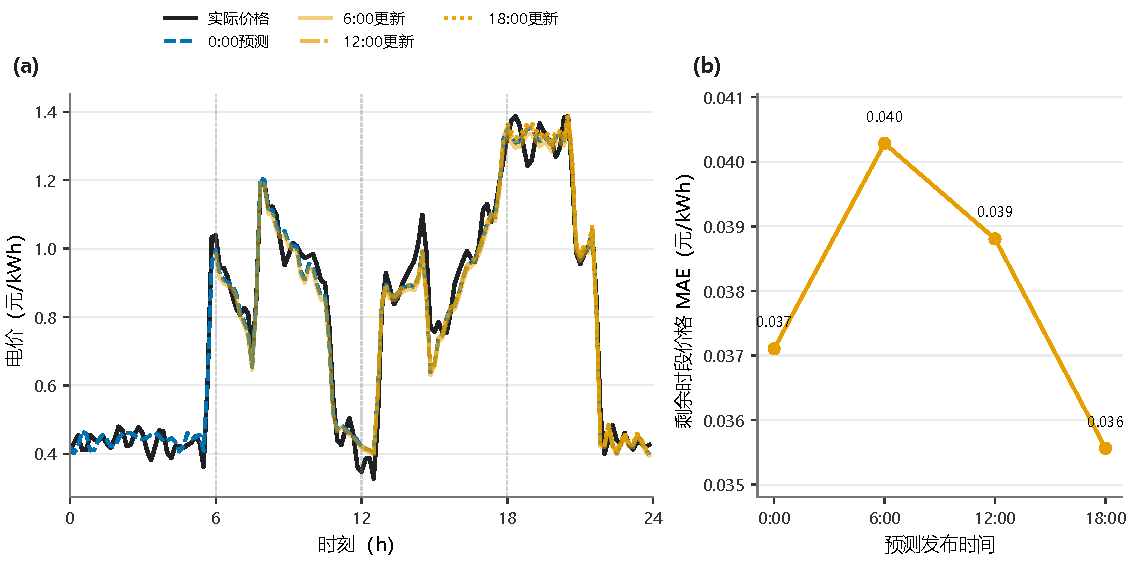
\includegraphics[width=.92\linewidth,height=7.0cm,keepaspectratio]{../new_figures_main/Q4_F2_price_forecast_update.pdf}
\caption{实际电价与各发布时间的预测对比}
\figtabnote{更新仅使用发布时间之前的实际电价。}
\end{figure}
\subsection{7.2 统计期费用与信息价值}
\begin{table}[H]\centering
\fontsize{9.5}{12}\selectfont\setlength{\tabcolsep}{4pt}\renewcommand{\arraystretch}{1.12}
\begin{adjustbox}{max width=\linewidth}\begin{tabular}{lcc}\toprule
\textbf{指标} & \textbf{问题四之二} & \textbf{问题四之三}\\\midrule
统计天数/d & 334 & 334\\
计划购电费/元 & 13603509.03 & 13068665.06\\
调整费/元 & 0.00 & 766977.43\\
紧急购电费/元 & 798263.55 & 117818.44\\
总费用/元 & 14401772.58 & 13953460.93\\
0时计划购电量/kWh & 20642939.91 & 20090653.88\\
最终计划购电量/kWh & 20642939.91 & 20535635.37\\
紧急购电量/kWh & 126055.49 & 22900.97\\
发生紧急购电天数/d & 103 & 91\\
余电量/kWh & 1668540.82 & 1421673.17\\
\bottomrule\end{tabular}\end{adjustbox}
\caption{波动电价下两种因果方案的统计期结果}
\end{table}
在实际电价结算下，因果日前方案费用为14401772.58元，因果滚动方案为13953460.93元，节约448311.65元，即3.11\%；紧急购电量分别为126055.49和22900.97 kWh，减少81.83\%。其储电范围仍为1200—10800 kWh，最大微网侧时段充、放电量均不超过833.33 kWh。
\par
\begin{table}[H]\centering
\fontsize{9.5}{12}\selectfont\setlength{\tabcolsep}{4pt}\renewcommand{\arraystretch}{1.12}
\begin{adjustbox}{max width=\linewidth}\begin{tabular}{lcc}\toprule
\textbf{信息条件} & \textbf{日前方案} & \textbf{滚动方案}\\\midrule
固定电价决策 & 1444.88 & 1399.16\\
因果价格预测 & 1440.18 & 1395.35\\
预知未来电价 & 1434.63 & 1385.41\\
完美信息基准 & 1280.93 & 同一基准\\
\bottomrule\end{tabular}\end{adjustbox}
\caption{统一按实际电价结算的价格信息对照（万元）}
\end{table}
为分开评价价格信息和供给信息，设置四种条件：固定价格决策使用附件1价格但仍按附件4结算；因果预测仅使用当时可知价格；预知电价方案知道当天未来价格，但负载和光伏仍按因果方式预测；完美信息基准同时知道实际负载、光伏和价格。相对固定价格决策，因果预测使日前和滚动方案分别节约0.33\%和0.27\%；进一步预知电价则在因果方案基础上再节约0.39\%和0.71\%。这些差额来自同一实际价格环境中的对照计算，不代表可实现的市场收益承诺。
\par
完美信息基准费用为12809266.07元，仅用于展示信息充分条件下的参考表现。它与因果策略的逐日状态和终端处理存在区别，没有证明对所有可行因果策略构成严格费用下界。
\par
\subsection{7.3 典型日期的对应结果}
\begin{table}[H]\centering
\fontsize{9.5}{12}\selectfont\setlength{\tabcolsep}{4pt}\renewcommand{\arraystretch}{1.12}
\begin{adjustbox}{max width=\linewidth}\begin{tabular}{lccccc}\toprule
\textbf{日期} & \textbf{方案} & \shortstack{\textbf{原计划}\\{\normalfont （kWh）}} & \shortstack{\textbf{最终计划}\\{\normalfont （kWh）}} & \shortstack{\textbf{总费用}\\{\normalfont （元）}} & \shortstack{\textbf{紧急购电}\\{\normalfont （kWh）}}\\\midrule
03-20 & 日前 & 66219.79 & 66219.79 & 42083.51 & 0.00\\
03-20 & 滚动 & 64782.09 & 65664.91 & 45045.32 & 251.85\\
06-21 & 日前 & 33748.13 & 33748.13 & 17278.64 & 0.00\\
06-21 & 滚动 & 33488.12 & 34062.20 & 17432.29 & 0.00\\
09-23 & 日前 & 66834.10 & 66834.10 & 44970.74 & 67.16\\
09-23 & 滚动 & 64822.50 & 68353.96 & 48268.01 & 7.77\\
12-21 & 日前 & 84525.79 & 84525.79 & 67455.10 & 0.00\\
12-21 & 滚动 & 83961.70 & 84524.30 & 68102.79 & 0.00\\
\bottomrule\end{tabular}\end{adjustbox}
\caption{波动电价下典型日购电与费用汇总}
\end{table}
为展示波动电价后的时段安排，表中“日前”对应问题四之二，“滚动”对应问题四之三；购电取最终执行量，原计划与所有逐时调整仍完整保存在相应结果工作簿中。
\par
\begin{table}[H]\centering
\fontsize{9.5}{12}\selectfont\setlength{\tabcolsep}{4pt}\renewcommand{\arraystretch}{1.12}
\begin{adjustbox}{max width=\linewidth}\begin{tabular}{lccccc}\toprule
\textbf{时间段} & \textbf{方案} & \textbf{03-20} & \textbf{06-21} & \textbf{09-23} & \textbf{12-21}\\\midrule
10:00–10:10 & 日前 & 0.00 & 0.00 & 0.00 & 0.00\\
10:00–10:10 & 滚动 & 0.00 & 0.00 & 0.00 & 0.00\\
\addlinespace[2pt]
12:00–12:10 & 日前 & 625.40 & 0.00 & 439.89 & 856.43\\
12:00–12:10 & 滚动 & 618.49 & 0.00 & 0.00 & 865.61\\
\addlinespace[2pt]
14:00–14:10 & 日前 & 0.00 & 0.00 & 0.00 & 0.00\\
14:00–14:10 & 滚动 & 0.00 & 0.00 & 0.00 & 0.00\\
\addlinespace[2pt]
16:00–16:10 & 日前 & 465.12 & 137.16 & 527.13 & 813.89\\
16:00–16:10 & 滚动 & 538.26 & 128.77 & 586.22 & 847.49\\
\addlinespace[2pt]
18:00–18:10 & 日前 & 671.07 & 13.22 & 0.00 & 729.95\\
18:00–18:10 & 滚动 & 671.07 & 0.00 & 0.00 & 439.00\\
\addlinespace[2pt]
20:00–20:10 & 日前 & 692.15 & 0.00 & 3.63 & 0.00\\
20:00–20:10 & 滚动 & 694.56 & 0.00 & 7.30 & 0.00\\
\bottomrule\end{tabular}\end{adjustbox}
\caption{波动电价下指定10分钟时段最终购电量（kWh）}
\end{table}
\begin{table}[H]\centering
\fontsize{9.5}{12}\selectfont\setlength{\tabcolsep}{4pt}\renewcommand{\arraystretch}{1.12}
\begin{adjustbox}{max width=\linewidth}\begin{tabular}{lccccc}\toprule
\textbf{时间段} & \textbf{方案} & \textbf{03-20} & \textbf{06-21} & \textbf{09-23} & \textbf{12-21}\\\midrule
00:00–04:00 & 日前 & 6653.96 / 247.10 & 166.36 / 1006.41 & 6284.54 / 30.55 & 507.30 / 229.56\\
00:00–04:00 & 滚动 & 6642.55 / 64.13 & 216.13 / 1014.16 & 6123.17 / 27.37 & 686.52 / 225.83\\
\addlinespace[2pt]
04:00–08:00 & 日前 & 2694.12 / 5133.41 & 1658.56 / 1755.02 & 4136.82 / 5339.30 & 316.74 / 971.38\\
04:00–08:00 & 滚动 & 1920.71 / 5713.74 & 2113.23 / 1371.89 & 4697.30 / 4162.08 & 326.01 / 1215.06\\
\addlinespace[2pt]
08:00–12:00 & 日前 & 5100.87 / 2777.38 & 10154.81 / 0.00 & 3930.46 / 1896.62 & 5011.80 / 6682.35\\
08:00–12:00 & 滚动 & 2904.15 / 2525.53 & 9663.15 / 0.00 & 5237.99 / 1896.62 & 5016.64 / 7135.31\\
\addlinespace[2pt]
12:00–16:00 & 日前 & 4594.71 / 527.79 & 0.00 / 0.00 & 4607.12 / 645.85 & 7318.90 / 2434.25\\
12:00–16:00 & 滚动 & 7112.77 / 254.72 & 0.00 / 0.00 & 1263.59 / 421.50 & 8000.11 / 2251.40\\
\addlinespace[2pt]
16:00–20:00 & 日前 & 27.96 / 6612.76 & 59.27 / 5157.66 & 24.02 / 5705.14 & 88.40 / 5307.03\\
16:00–20:00 & 滚动 & 115.61 / 6197.15 & 46.92 / 5317.66 & 110.62 / 5701.61 & 0.00 / 5621.03\\
\addlinespace[2pt]
20:00–24:00 & 日前 & 1201.75 / 1766.24 & 1410.14 / 2621.53 & 493.21 / 2595.02 & 452.32 / 3006.59\\
20:00–24:00 & 滚动 & 1176.75 / 1737.37 & 1340.32 / 2659.30 & 450.37 / 2668.98 & 445.38 / 2961.01\\
\addlinespace[2pt]
日初 / 日末 & 日前 & 3008.05 / 2293.32 & 3086.50 / 3478.93 & 2063.73 / 1578.42 & 10408.89 / 2033.49\\
日初 / 日末 & 滚动 & 2719.07 / 2279.19 & 2657.91 / 3185.22 & 2061.60 / 1625.04 & 10204.32 / 1665.23\\
\bottomrule\end{tabular}\end{adjustbox}
\caption{波动电价下典型日储能量（kWh）}
\figtabnote{单元格依次列出充电量与放电量；末两行为日初和日末储电量。}
\end{table}
\begin{table}[H]\centering
\fontsize{9.5}{12}\selectfont\setlength{\tabcolsep}{4pt}\renewcommand{\arraystretch}{1.12}
\begin{adjustbox}{max width=\linewidth}\begin{tabular}{lccccccc}\toprule
\multicolumn{2}{c}{\textbf{03-20}} & \multicolumn{2}{c}{\textbf{06-21}} & \multicolumn{2}{c}{\textbf{09-23}} & \multicolumn{2}{c}{\textbf{12-21}}\\
\cmidrule(lr){1-2} \cmidrule(lr){3-4} \cmidrule(lr){5-6} \cmidrule(lr){7-8}
\textbf{时段} & \shortstack{\textbf{购电量}\\{\normalfont （kWh）}} & \textbf{时段} & \shortstack{\textbf{购电量}\\{\normalfont （kWh）}} & \textbf{时段} & \shortstack{\textbf{购电量}\\{\normalfont （kWh）}} & \textbf{时段} & \shortstack{\textbf{购电量}\\{\normalfont （kWh）}}\\\midrule
无 & 0.00 & 无 & 0.00 & 20:10–20:20 & 10.00 & 无 & 0.00\\
— & — & — & — & 21:00–21:10 & 5.66 & — & —\\
— & — & — & — & 21:20–21:40 & 51.50 & — & —\\
合计 & 0.00 & 合计 & 0.00 & 合计 & 67.16 & 合计 & 0.00\\
\bottomrule\end{tabular}\end{adjustbox}
\caption{问题四之二四个典型日紧急购电（kWh）}
\end{table}
\begin{table}[H]\centering
\fontsize{9.5}{12}\selectfont\setlength{\tabcolsep}{4pt}\renewcommand{\arraystretch}{1.12}
\begin{adjustbox}{max width=\linewidth}\begin{tabular}{lccccccc}\toprule
\multicolumn{2}{c}{\textbf{03-20}} & \multicolumn{2}{c}{\textbf{06-21}} & \multicolumn{2}{c}{\textbf{09-23}} & \multicolumn{2}{c}{\textbf{12-21}}\\
\cmidrule(lr){1-2} \cmidrule(lr){3-4} \cmidrule(lr){5-6} \cmidrule(lr){7-8}
\textbf{时段} & \shortstack{\textbf{购电量}\\{\normalfont （kWh）}} & \textbf{时段} & \shortstack{\textbf{购电量}\\{\normalfont （kWh）}} & \textbf{时段} & \shortstack{\textbf{购电量}\\{\normalfont （kWh）}} & \textbf{时段} & \shortstack{\textbf{购电量}\\{\normalfont （kWh）}}\\\midrule
09:10–10:00 & 251.85 & 无 & 0.00 & 20:10–20:20 & 7.77 & 无 & 0.00\\
合计 & 251.85 & 合计 & 0.00 & 合计 & 7.77 & 合计 & 0.00\\
\bottomrule\end{tabular}\end{adjustbox}
\caption{问题四之三四个典型日紧急购电（kWh）}
\end{table}
\subsection{7.4 保持日均价格的波动灵敏度}
直接放大价格会同时改变平均购电成本和波动强度，难以区分二者作用。因此以每日电价的对数偏离构造压力情形，并保持每日算术平均价不变：
\par
\begin{equation}
u_{i,t}^{(\lambda)}=\exp\{\lambda(\log\pi_{i,t}-\overline{\log\pi_i})\},\qquad
\pi_{i,t}^{(\lambda)}=\overline\pi_i\frac{u_{i,t}^{(\lambda)}}{\overline{u_i^{(\lambda)}}}. \tag{19}
\end{equation}
其中横线表示日内144个时段的算术平均，$\lambda$取0.50、0.75、1.00、1.25、1.50。每个压力情形分别根据其历史数据形成因果价格预测，再连续运行全年；不是将原购电计划简单乘上新价格。$\lambda=1$恢复原实际电价并复现主结果。
\par
\begin{table}[H]\centering
\fontsize{9.5}{12}\selectfont\setlength{\tabcolsep}{4pt}\renewcommand{\arraystretch}{1.12}
\begin{adjustbox}{max width=\linewidth}\begin{tabular}{lccccc}\toprule
\textbf{$\lambda$} & \textbf{日内CV均值} & \shortstack{\textbf{日前费用}\\{\normalfont （万元）}} & \shortstack{\textbf{滚动费用}\\{\normalfont （万元）}} & \shortstack{\textbf{节约}\\{\normalfont （万元）}} & \textbf{节约率}\\\midrule
0.50 & 0.219 & 1536.67 & 1518.63 & 18.04 & 1.17\%\\
0.75 & 0.324 & 1490.03 & 1457.99 & 32.04 & 2.15\%\\
1.00 & 0.425 & 1440.18 & 1395.35 & 44.83 & 3.11\%\\
1.25 & 0.522 & 1392.11 & 1338.74 & 53.37 & 3.83\%\\
1.50 & 0.615 & 1352.40 & 1288.06 & 64.34 & 4.76\%\\
\bottomrule\end{tabular}\end{adjustbox}
\caption{保持日均价格的波动试验}
\end{table}
在本组五个情形中，滚动方案费用始终较低，节约率由1.17\%升至4.76\%；日内价格变异系数均值由0.219升至0.615。保持日均价并不意味着各策略的总费用不变，因为购电量与价格的时段配合发生变化。该构造表明所给数据中更强的峰谷差为调整与储能提供了更大价值，但未证明对任意价格过程均单调改善。
\par
\begin{figure}[H]\centering
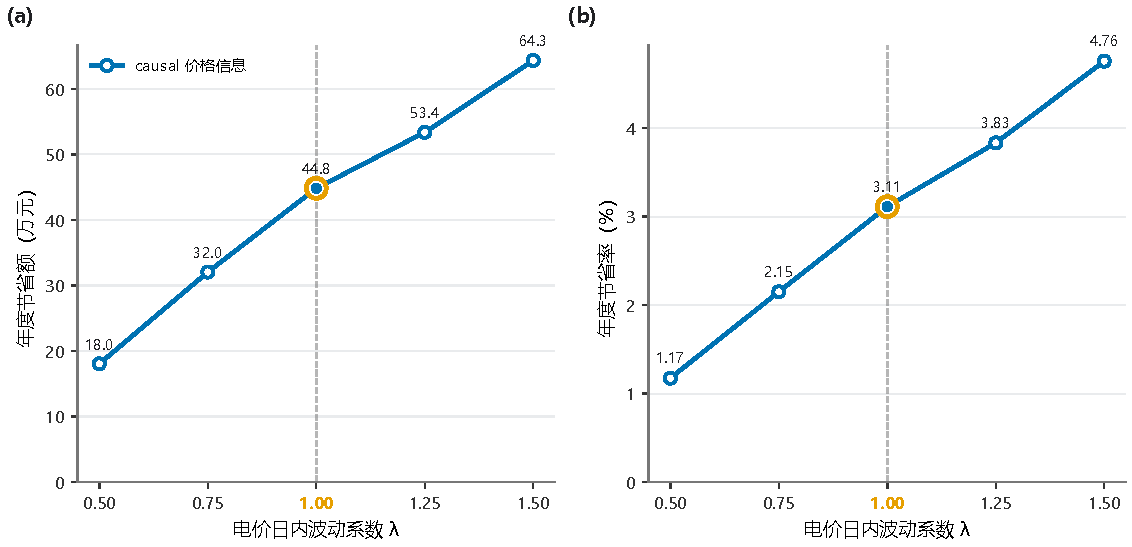
\includegraphics[width=.92\linewidth,height=7.0cm,keepaspectratio]{../new_figures_main/Q4_F4_rolling_gain_sensitivity.pdf}
\caption{不同电价波动情形下滚动策略的节约效果}
\figtabnote{保持日均价的五种波动情形下，滚动策略相对日前策略的费用节约与节约率。}
\end{figure}
\section{8 模型检验与结果边界}
\subsection{8.1 预测检验和约束检验}
预测指标在实际观测出现后计算，评价日$t$的预测时不把该日尚未发生的观测提供给模型。设对应评价样本数为$M$，则
\par
\begin{equation}
\mathrm{MAE}=\frac1M\sum_{j=1}^M|\widehat P_j-P_j|,\qquad
\mathrm{RMSE}=\sqrt{\frac1M\sum_{j=1}^M(\widehat P_j-P_j)^2}. \tag{20}
\end{equation}
光伏包含大量零值，本文不采用以实际功率为分母的MAPE，避免夜间零值导致指标失真。各发布时间只统计当日尚未执行的时段，表中误差只宜在同一发布时间下比较方法。
\par
\begin{table}[H]\centering
\fontsize{9.5}{12}\selectfont\setlength{\tabcolsep}{4pt}\renewcommand{\arraystretch}{1.12}
\begin{adjustbox}{max width=\linewidth}\begin{tabular}{lcc}\toprule
\textbf{检验项目} & \textbf{结果} & \textbf{结论范围}\\\midrule
问题一原记录最大平衡残差 & $2.27\times10^{-13}$ kWh & 给定确定性实例\\
问题二至四原记录最大平衡残差 & $2.27\times10^{-13}$ kWh & 主方案实际运行\\
独立重算电量平衡最大残差 & $4.55\times10^{-13}$ kWh & 全部23份缓存\\
独立重算SOC递推最大残差 & $9.09\times10^{-13}$ kWh & 全部23份缓存\\
储电量物理范围 & 1200—10800 kWh & 主方案及已计算对照\\
问题二至四时段充放电上限 & 833.3333 kWh & 微网侧\\
同时充放电时段数 & 0 & 实际运行轨迹\\
跨日储电量 & 连续衔接 & 含1月预热段\\
工作簿购电量与缓存最大差 & $4.55\times10^{-13}$ kWh & 四份统计期结果\\
波动试验每日均价最大误差 & $1.23\times10^{-15}$ 元/kWh以内 & 五种波动情形\\
\bottomrule\end{tabular}\end{adjustbox}
\caption{实际运行与数值结果核验}
\end{table}
电量平衡残差按实际轨迹直接重算；不同浮点运算顺序使独立重算与原记录的末位略有差异，均低于$10^{-12}$ kWh。跨日检验包括1月份预热段到2月份统计段的衔接。统计期计划购电、调整费用和紧急费用分别求和后，再与JSON汇总及结果工作簿核对。所有表格先对未舍入的时段数据求和，再保留两位小数，不能以表中四舍五入值重新求和要求逐分一致。
\par
问题一未显式施加充放电互斥约束，但给定实例的最优解没有同时充放电。问题二至四的实际运行规则保证互斥；规划场景采用连续线性模型，不将实际轨迹的验证推广成任意场景、任意参数下的普遍定理。
\par
\subsection{8.2 结论的可支持范围}
本研究完成了物理约束检查、因果信息检查、策略消融、容量与功率灵敏度以及电价波动试验。没有重新开展效率扫描、场景数量扫描或参数最优调参，也没有把当前费用与未计算的确定性MPC作定量比较。单年的滚动回测能够说明本数据上的运行效果，不能替代多年度外部样本验证。
\par
同样，完美信息计算只作为基准；经验分位带只描述有限场景；费用差额只说明被比较方案的差异。对这些概念作明确限定，才能使“预测改善”“风险降低”和“策略节约”分别有与其相称的证据。
\par
\section{9 模型评价与应用建议}
\subsection{9.1 模型优点}
模型把购电承诺、预报更新和实时供电分开处理，能直接体现普通购电、调整和五倍紧急购电的不同代价。连续线性结构使时段储能约束、历史场景和调整费用可以在同一优化框架中求解，便于逐项检查。历史配对残差无需另行假设概率分布，实际运行又只使用当前及过去观测，因此结果可以沿时间顺序复核。
\par
对于额外预报的价值，模型同时报告费用和紧急购电量，并用有限方案消融显示二者的取舍。波动价格部分区分预测与结算，也区分只预知价格和全部供给信息，使不同信息条件的结果具有明确含义。
\par
\subsection{9.2 模型不足与可行改进}
首先，问题一和后续问题的储能功率计量侧不同。若进一步用于设备调度，应先依据设备铭牌明确交流侧或储能侧上限，再统一所有模型和结果重新计算；当前论文保留原有计算的前提和数值，不用变量换名掩盖该差异。
\par
其次，十日残差与固定安全裕度对极端偏差的覆盖有限。两阶段场景决策比逐时实际信息更充分，也会低估某些适应困难。可在增加历史样本后检验场景数和裕度的取舍，但现有证据不足以指定新的最优值。
\par
再次，光伏比例修正在6时和12时增加了平均误差。后续可用仅由历史数据确定的启用条件筛选修正，或限制比例幅度；其效果需要重新回测，本文不预报改进幅度。电价比例修正只能改变整体水平，无法预测峰谷移动，适用范围也受此限制。
\par
最后，模型忽略储能寿命和额外交易规则，0.42元/kWh终端价值为固定经验值，不能替代长期设备经济性分析。实际应用应在本题能量调度框架上补充这些信息，而不是直接按购电费最低结果进行设备投资。
\par
\subsection{9.3 调控结论}
在给定计量约定下，问题一可用线性规划得到日内闭合的购电与储能计划，费用为35101.57元。负载和光伏不确定时，残差场景与因果储能调度给出可执行日前计划；增加日内调整后，统计期总费用由1370.17万元降至1326.66万元，紧急购电量由12.79万kWh降至2.12万kWh。
\par
若以已有试验的费用为主要选择依据，可采用12、18时调整方案；完整追索式主方案提供较低的紧急购电量，但需要更多费用。实际电价波动下，因果滚动方案较对应日前方案节约44.83万元。在全部结论中，时段供电由购电与储能共同保障，策略优劣由实际结算与实际轨迹评价，而非仅由预测误差或优化器状态决定。
\par
\clearpage
\section{参考文献}
{\small\noindent\hangindent=2em [1] OLIVARES D E, MEHRIZI-SANI A, ETEMADI A H, et al. Trends in microgrid control[J]. IEEE Transactions on Smart Grid, 2014, 5(4): 1905–1919. DOI: \href{https://doi.org/10.1109/TSG.2013.2295514}{10.1109/TSG.2013.2295514}.\par}\vspace{4pt}
{\small\noindent\hangindent=2em [2] BIRGE J R, LOUVEAUX F. Introduction to Stochastic Programming[M]. 2nd ed. New York: Springer, 2011. DOI: \href{https://doi.org/10.1007/978-1-4614-0237-4}{10.1007/978-1-4614-0237-4}.\par}\vspace{4pt}
{\small\noindent\hangindent=2em [3] PALMA-BEHNKE R, BENAVIDES C, LANAS F, et al. A microgrid energy management system based on the rolling horizon strategy[J]. IEEE Transactions on Smart Grid, 2013, 4(2): 996–1006. DOI: \href{https://doi.org/10.1109/TSG.2012.2231440}{10.1109/TSG.2012.2231440}.\par}\vspace{4pt}
{\small\noindent\hangindent=2em [4] HYNDMAN R J, ATHANASOPOULOS G. Forecasting: Principles and Practice[M/OL]. 3rd ed. Melbourne: OTexts, 2021[2026-09-13]. \href{https://otexts.com/fpp3/}{在线版本}.\par}\vspace{4pt}
{\small\noindent\hangindent=2em [5] VIRTANEN P, GOMMERS R, OLIPHANT T E, et al. SciPy 1.0: fundamental algorithms for scientific computing in Python[J]. Nature Methods, 2020, 17(3): 261–272. DOI: \href{https://doi.org/10.1038/s41592-019-0686-2}{10.1038/s41592-019-0686-2}.\par}\vspace{4pt}
{\small\noindent\hangindent=2em [6] HUANGFU Q, HALL J A J. Parallelizing the dual revised simplex method[J]. Mathematical Programming Computation, 2018, 10(1): 119–142. DOI: \href{https://doi.org/10.1007/s12532-017-0130-5}{10.1007/s12532-017-0130-5}.\par}\vspace{4pt}
\clearpage
\section{附录 A 支撑材料文件清单与结果说明}
完整144时段结果见随附的result1.xlsx、result2.xlsx、result3.xlsx、result4-2.xlsx、result4-3.xlsx。问题二至四覆盖2月1日至12月31日；问题三和问题四之三同时提供0时计划及更新后的购电量。正文典型日表由既有JSON中的未舍入数组直接生成，紧急购电将相邻非零时段合并列示。
\par
支撑材料统一保存于backing\_material.zip，包含76个文件，完整清单见表A1，所有路径均相对压缩包根目录。完整Python程序位于根目录run\_all.py、plot\_style.py及src目录，依赖清单为requirements-final.txt。根目录的五份Excel为已填结果，data/附件/附件5目录中的同名文件为空白输出模板。复现时应解压至独立目录，按说明.md及原运行入口执行。
\par
主文使用6幅原始结果图，并新增1幅概括现有模型关系的流程图；其余原始图随原仓库保留。原图中含“理论下界”字样的策略图未纳入本文，相关比较改用数值表，并统一采用“完美信息基准”名称。各模型的原始输出名称保持不变。
\par
\begingroup\fontsize{9.5}{12}\selectfont\renewcommand{\arraystretch}{1.15}
\begin{longtable}{@{}>{\raggedright\arraybackslash}p{0.57\linewidth}>{\raggedright\arraybackslash}p{0.39\linewidth}@{}}
\toprule 文件名 & 用途\\\midrule\endfirsthead
\toprule 文件名 & 用途\\\midrule\endhead
\midrule\multicolumn{2}{r}{续下页}\\\endfoot\bottomrule\endlastfoot
F\allowbreak{}I\allowbreak{}N\allowbreak{}A\allowbreak{}L\allowbreak{}\_\allowbreak{}D\allowbreak{}E\allowbreak{}L\allowbreak{}I\allowbreak{}V\allowbreak{}E\allowbreak{}R\allowbreak{}Y\allowbreak{}\_\allowbreak{}A\allowbreak{}U\allowbreak{}D\allowbreak{}I\allowbreak{}T\allowbreak{}.\allowbreak{}m\allowbreak{}d\allowbreak{} & 原清单程序需要的历史来源记录；不作为本次打包验收结论\\
S\allowbreak{}O\allowbreak{}U\allowbreak{}R\allowbreak{}C\allowbreak{}E\allowbreak{}\_\allowbreak{}H\allowbreak{}A\allowbreak{}S\allowbreak{}H\allowbreak{}E\allowbreak{}S\allowbreak{}.\allowbreak{}m\allowbreak{}d\allowbreak{} & 原清单程序需要的历史来源记录；不作为本次打包验收结论\\
c\allowbreak{}建\allowbreak{}模\allowbreak{}说\allowbreak{}明\allowbreak{}与\allowbreak{}结\allowbreak{}果\allowbreak{}.\allowbreak{}t\allowbreak{}x\allowbreak{}t\allowbreak{} & 建模说明的旧名称兼容副本，供原清单脚本读取\\
d\allowbreak{}a\allowbreak{}t\allowbreak{}a\allowbreak{}/\allowbreak{}附\allowbreak{}件\allowbreak{}/\allowbreak{}附\allowbreak{}件\allowbreak{}1\allowbreak{}.\allowbreak{}x\allowbreak{}l\allowbreak{}s\allowbreak{}x\allowbreak{} & 题目原始输入附件；保持原文件及原属性不变\\
d\allowbreak{}a\allowbreak{}t\allowbreak{}a\allowbreak{}/\allowbreak{}附\allowbreak{}件\allowbreak{}/\allowbreak{}附\allowbreak{}件\allowbreak{}2\allowbreak{}.\allowbreak{}x\allowbreak{}l\allowbreak{}s\allowbreak{}x\allowbreak{} & 题目原始输入附件；保持原文件及原属性不变\\
d\allowbreak{}a\allowbreak{}t\allowbreak{}a\allowbreak{}/\allowbreak{}附\allowbreak{}件\allowbreak{}/\allowbreak{}附\allowbreak{}件\allowbreak{}3\allowbreak{}.\allowbreak{}x\allowbreak{}l\allowbreak{}s\allowbreak{}x\allowbreak{} & 题目原始输入附件；保持原文件及原属性不变\\
d\allowbreak{}a\allowbreak{}t\allowbreak{}a\allowbreak{}/\allowbreak{}附\allowbreak{}件\allowbreak{}/\allowbreak{}附\allowbreak{}件\allowbreak{}4\allowbreak{}.\allowbreak{}x\allowbreak{}l\allowbreak{}s\allowbreak{}x\allowbreak{} & 题目原始输入附件；保持原文件及原属性不变\\
d\allowbreak{}a\allowbreak{}t\allowbreak{}a\allowbreak{}/\allowbreak{}附\allowbreak{}件\allowbreak{}/\allowbreak{}附\allowbreak{}件\allowbreak{}5\allowbreak{}/\allowbreak{}r\allowbreak{}e\allowbreak{}s\allowbreak{}u\allowbreak{}l\allowbreak{}t\allowbreak{}1\allowbreak{}.\allowbreak{}x\allowbreak{}l\allowbreak{}s\allowbreak{}x\allowbreak{} & 附件5空白输出模板，仅供程序生成结果使用\\
d\allowbreak{}a\allowbreak{}t\allowbreak{}a\allowbreak{}/\allowbreak{}附\allowbreak{}件\allowbreak{}/\allowbreak{}附\allowbreak{}件\allowbreak{}5\allowbreak{}/\allowbreak{}r\allowbreak{}e\allowbreak{}s\allowbreak{}u\allowbreak{}l\allowbreak{}t\allowbreak{}2\allowbreak{}.\allowbreak{}x\allowbreak{}l\allowbreak{}s\allowbreak{}x\allowbreak{} & 附件5空白输出模板，仅供程序生成结果使用\\
d\allowbreak{}a\allowbreak{}t\allowbreak{}a\allowbreak{}/\allowbreak{}附\allowbreak{}件\allowbreak{}/\allowbreak{}附\allowbreak{}件\allowbreak{}5\allowbreak{}/\allowbreak{}r\allowbreak{}e\allowbreak{}s\allowbreak{}u\allowbreak{}l\allowbreak{}t\allowbreak{}3\allowbreak{}.\allowbreak{}x\allowbreak{}l\allowbreak{}s\allowbreak{}x\allowbreak{} & 附件5空白输出模板，仅供程序生成结果使用\\
d\allowbreak{}a\allowbreak{}t\allowbreak{}a\allowbreak{}/\allowbreak{}附\allowbreak{}件\allowbreak{}/\allowbreak{}附\allowbreak{}件\allowbreak{}5\allowbreak{}/\allowbreak{}r\allowbreak{}e\allowbreak{}s\allowbreak{}u\allowbreak{}l\allowbreak{}t\allowbreak{}4\allowbreak{}-\allowbreak{}2\allowbreak{}.\allowbreak{}x\allowbreak{}l\allowbreak{}s\allowbreak{}x\allowbreak{} & 附件5空白输出模板，仅供程序生成结果使用\\
d\allowbreak{}a\allowbreak{}t\allowbreak{}a\allowbreak{}/\allowbreak{}附\allowbreak{}件\allowbreak{}/\allowbreak{}附\allowbreak{}件\allowbreak{}5\allowbreak{}/\allowbreak{}r\allowbreak{}e\allowbreak{}s\allowbreak{}u\allowbreak{}l\allowbreak{}t\allowbreak{}4\allowbreak{}-\allowbreak{}3\allowbreak{}.\allowbreak{}x\allowbreak{}l\allowbreak{}s\allowbreak{}x\allowbreak{} & 附件5空白输出模板，仅供程序生成结果使用\\
n\allowbreak{}e\allowbreak{}w\allowbreak{}\_\allowbreak{}f\allowbreak{}i\allowbreak{}g\allowbreak{}u\allowbreak{}r\allowbreak{}e\allowbreak{}s\allowbreak{}\_\allowbreak{}m\allowbreak{}a\allowbreak{}i\allowbreak{}n\allowbreak{}/\allowbreak{}Q\allowbreak{}1\allowbreak{}\_\allowbreak{}F\allowbreak{}1\allowbreak{}\_\allowbreak{}o\allowbreak{}p\allowbreak{}t\allowbreak{}i\allowbreak{}m\allowbreak{}a\allowbreak{}l\allowbreak{}\_\allowbreak{}d\allowbreak{}i\allowbreak{}s\allowbreak{}p\allowbreak{}a\allowbreak{}t\allowbreak{}c\allowbreak{}h\allowbreak{}.\allowbreak{}p\allowbreak{}n\allowbreak{}g\allowbreak{} & 现有计算结果图，保留原图\\
n\allowbreak{}e\allowbreak{}w\allowbreak{}\_\allowbreak{}f\allowbreak{}i\allowbreak{}g\allowbreak{}u\allowbreak{}r\allowbreak{}e\allowbreak{}s\allowbreak{}\_\allowbreak{}m\allowbreak{}a\allowbreak{}i\allowbreak{}n\allowbreak{}/\allowbreak{}Q\allowbreak{}1\allowbreak{}\_\allowbreak{}F\allowbreak{}2\allowbreak{}\_\allowbreak{}s\allowbreak{}o\allowbreak{}l\allowbreak{}u\allowbreak{}t\allowbreak{}i\allowbreak{}o\allowbreak{}n\allowbreak{}\_\allowbreak{}d\allowbreak{}i\allowbreak{}a\allowbreak{}g\allowbreak{}n\allowbreak{}o\allowbreak{}s\allowbreak{}t\allowbreak{}i\allowbreak{}c\allowbreak{}s\allowbreak{}.\allowbreak{}p\allowbreak{}n\allowbreak{}g\allowbreak{} & 现有计算结果图，保留原图\\
n\allowbreak{}e\allowbreak{}w\allowbreak{}\_\allowbreak{}f\allowbreak{}i\allowbreak{}g\allowbreak{}u\allowbreak{}r\allowbreak{}e\allowbreak{}s\allowbreak{}\_\allowbreak{}m\allowbreak{}a\allowbreak{}i\allowbreak{}n\allowbreak{}/\allowbreak{}Q\allowbreak{}1\allowbreak{}\_\allowbreak{}F\allowbreak{}3\allowbreak{}\_\allowbreak{}s\allowbreak{}t\allowbreak{}o\allowbreak{}r\allowbreak{}a\allowbreak{}g\allowbreak{}e\allowbreak{}\_\allowbreak{}s\allowbreak{}e\allowbreak{}n\allowbreak{}s\allowbreak{}i\allowbreak{}t\allowbreak{}i\allowbreak{}v\allowbreak{}i\allowbreak{}t\allowbreak{}y\allowbreak{}.\allowbreak{}p\allowbreak{}n\allowbreak{}g\allowbreak{} & 现有计算结果图，保留原图\\
n\allowbreak{}e\allowbreak{}w\allowbreak{}\_\allowbreak{}f\allowbreak{}i\allowbreak{}g\allowbreak{}u\allowbreak{}r\allowbreak{}e\allowbreak{}s\allowbreak{}\_\allowbreak{}m\allowbreak{}a\allowbreak{}i\allowbreak{}n\allowbreak{}/\allowbreak{}Q\allowbreak{}2\allowbreak{}\_\allowbreak{}F\allowbreak{}1\allowbreak{}\_\allowbreak{}t\allowbreak{}y\allowbreak{}p\allowbreak{}i\allowbreak{}c\allowbreak{}a\allowbreak{}l\allowbreak{}\_\allowbreak{}d\allowbreak{}i\allowbreak{}s\allowbreak{}p\allowbreak{}a\allowbreak{}t\allowbreak{}c\allowbreak{}h\allowbreak{}.\allowbreak{}p\allowbreak{}n\allowbreak{}g\allowbreak{} & 现有计算结果图，保留原图\\
n\allowbreak{}e\allowbreak{}w\allowbreak{}\_\allowbreak{}f\allowbreak{}i\allowbreak{}g\allowbreak{}u\allowbreak{}r\allowbreak{}e\allowbreak{}s\allowbreak{}\_\allowbreak{}m\allowbreak{}a\allowbreak{}i\allowbreak{}n\allowbreak{}/\allowbreak{}Q\allowbreak{}2\allowbreak{}\_\allowbreak{}F\allowbreak{}2\allowbreak{}\_\allowbreak{}u\allowbreak{}n\allowbreak{}c\allowbreak{}e\allowbreak{}r\allowbreak{}t\allowbreak{}a\allowbreak{}i\allowbreak{}n\allowbreak{}t\allowbreak{}y\allowbreak{}\_\allowbreak{}s\allowbreak{}c\allowbreak{}e\allowbreak{}n\allowbreak{}a\allowbreak{}r\allowbreak{}i\allowbreak{}o\allowbreak{}s\allowbreak{}.\allowbreak{}p\allowbreak{}n\allowbreak{}g\allowbreak{} & 现有计算结果图，保留原图\\
n\allowbreak{}e\allowbreak{}w\allowbreak{}\_\allowbreak{}f\allowbreak{}i\allowbreak{}g\allowbreak{}u\allowbreak{}r\allowbreak{}e\allowbreak{}s\allowbreak{}\_\allowbreak{}m\allowbreak{}a\allowbreak{}i\allowbreak{}n\allowbreak{}/\allowbreak{}Q\allowbreak{}2\allowbreak{}\_\allowbreak{}F\allowbreak{}3\allowbreak{}\_\allowbreak{}a\allowbreak{}n\allowbreak{}n\allowbreak{}u\allowbreak{}a\allowbreak{}l\allowbreak{}\_\allowbreak{}r\allowbreak{}i\allowbreak{}s\allowbreak{}k\allowbreak{}\_\allowbreak{}p\allowbreak{}r\allowbreak{}o\allowbreak{}f\allowbreak{}i\allowbreak{}l\allowbreak{}e\allowbreak{}.\allowbreak{}p\allowbreak{}n\allowbreak{}g\allowbreak{} & 现有计算结果图，保留原图\\
n\allowbreak{}e\allowbreak{}w\allowbreak{}\_\allowbreak{}f\allowbreak{}i\allowbreak{}g\allowbreak{}u\allowbreak{}r\allowbreak{}e\allowbreak{}s\allowbreak{}\_\allowbreak{}m\allowbreak{}a\allowbreak{}i\allowbreak{}n\allowbreak{}/\allowbreak{}Q\allowbreak{}3\allowbreak{}\_\allowbreak{}F\allowbreak{}1\allowbreak{}\_\allowbreak{}r\allowbreak{}o\allowbreak{}l\allowbreak{}l\allowbreak{}i\allowbreak{}n\allowbreak{}g\allowbreak{}\_\allowbreak{}t\allowbreak{}i\allowbreak{}m\allowbreak{}e\allowbreak{}l\allowbreak{}i\allowbreak{}n\allowbreak{}e\allowbreak{}.\allowbreak{}p\allowbreak{}n\allowbreak{}g\allowbreak{} & 现有计算结果图，保留原图\\
n\allowbreak{}e\allowbreak{}w\allowbreak{}\_\allowbreak{}f\allowbreak{}i\allowbreak{}g\allowbreak{}u\allowbreak{}r\allowbreak{}e\allowbreak{}s\allowbreak{}\_\allowbreak{}m\allowbreak{}a\allowbreak{}i\allowbreak{}n\allowbreak{}/\allowbreak{}Q\allowbreak{}3\allowbreak{}\_\allowbreak{}F\allowbreak{}2\allowbreak{}\_\allowbreak{}f\allowbreak{}o\allowbreak{}r\allowbreak{}e\allowbreak{}c\allowbreak{}a\allowbreak{}s\allowbreak{}t\allowbreak{}\_\allowbreak{}i\allowbreak{}m\allowbreak{}p\allowbreak{}r\allowbreak{}o\allowbreak{}v\allowbreak{}e\allowbreak{}m\allowbreak{}e\allowbreak{}n\allowbreak{}t\allowbreak{}.\allowbreak{}p\allowbreak{}n\allowbreak{}g\allowbreak{} & 现有计算结果图，保留原图\\
n\allowbreak{}e\allowbreak{}w\allowbreak{}\_\allowbreak{}f\allowbreak{}i\allowbreak{}g\allowbreak{}u\allowbreak{}r\allowbreak{}e\allowbreak{}s\allowbreak{}\_\allowbreak{}m\allowbreak{}a\allowbreak{}i\allowbreak{}n\allowbreak{}/\allowbreak{}Q\allowbreak{}3\allowbreak{}\_\allowbreak{}F\allowbreak{}3\allowbreak{}\_\allowbreak{}s\allowbreak{}t\allowbreak{}r\allowbreak{}a\allowbreak{}t\allowbreak{}e\allowbreak{}g\allowbreak{}y\allowbreak{}\_\allowbreak{}p\allowbreak{}a\allowbreak{}r\allowbreak{}e\allowbreak{}t\allowbreak{}o\allowbreak{}.\allowbreak{}p\allowbreak{}n\allowbreak{}g\allowbreak{} & 现有计算结果图，保留原图\\
n\allowbreak{}e\allowbreak{}w\allowbreak{}\_\allowbreak{}f\allowbreak{}i\allowbreak{}g\allowbreak{}u\allowbreak{}r\allowbreak{}e\allowbreak{}s\allowbreak{}\_\allowbreak{}m\allowbreak{}a\allowbreak{}i\allowbreak{}n\allowbreak{}/\allowbreak{}Q\allowbreak{}3\allowbreak{}\_\allowbreak{}F\allowbreak{}4\allowbreak{}\_\allowbreak{}p\allowbreak{}l\allowbreak{}a\allowbreak{}n\allowbreak{}\_\allowbreak{}e\allowbreak{}v\allowbreak{}o\allowbreak{}l\allowbreak{}u\allowbreak{}t\allowbreak{}i\allowbreak{}o\allowbreak{}n\allowbreak{}.\allowbreak{}p\allowbreak{}n\allowbreak{}g\allowbreak{} & 现有计算结果图，保留原图\\
n\allowbreak{}e\allowbreak{}w\allowbreak{}\_\allowbreak{}f\allowbreak{}i\allowbreak{}g\allowbreak{}u\allowbreak{}r\allowbreak{}e\allowbreak{}s\allowbreak{}\_\allowbreak{}m\allowbreak{}a\allowbreak{}i\allowbreak{}n\allowbreak{}/\allowbreak{}Q\allowbreak{}4\allowbreak{}\_\allowbreak{}F\allowbreak{}1\allowbreak{}\_\allowbreak{}i\allowbreak{}n\allowbreak{}f\allowbreak{}o\allowbreak{}r\allowbreak{}m\allowbreak{}a\allowbreak{}t\allowbreak{}i\allowbreak{}o\allowbreak{}n\allowbreak{}\_\allowbreak{}v\allowbreak{}a\allowbreak{}l\allowbreak{}u\allowbreak{}e\allowbreak{}.\allowbreak{}p\allowbreak{}n\allowbreak{}g\allowbreak{} & 现有计算结果图，保留原图\\
n\allowbreak{}e\allowbreak{}w\allowbreak{}\_\allowbreak{}f\allowbreak{}i\allowbreak{}g\allowbreak{}u\allowbreak{}r\allowbreak{}e\allowbreak{}s\allowbreak{}\_\allowbreak{}m\allowbreak{}a\allowbreak{}i\allowbreak{}n\allowbreak{}/\allowbreak{}Q\allowbreak{}4\allowbreak{}\_\allowbreak{}F\allowbreak{}2\allowbreak{}\_\allowbreak{}p\allowbreak{}r\allowbreak{}i\allowbreak{}c\allowbreak{}e\allowbreak{}\_\allowbreak{}f\allowbreak{}o\allowbreak{}r\allowbreak{}e\allowbreak{}c\allowbreak{}a\allowbreak{}s\allowbreak{}t\allowbreak{}\_\allowbreak{}u\allowbreak{}p\allowbreak{}d\allowbreak{}a\allowbreak{}t\allowbreak{}e\allowbreak{}.\allowbreak{}p\allowbreak{}n\allowbreak{}g\allowbreak{} & 现有计算结果图，保留原图\\
n\allowbreak{}e\allowbreak{}w\allowbreak{}\_\allowbreak{}f\allowbreak{}i\allowbreak{}g\allowbreak{}u\allowbreak{}r\allowbreak{}e\allowbreak{}s\allowbreak{}\_\allowbreak{}m\allowbreak{}a\allowbreak{}i\allowbreak{}n\allowbreak{}/\allowbreak{}Q\allowbreak{}4\allowbreak{}\_\allowbreak{}F\allowbreak{}3\allowbreak{}\_\allowbreak{}p\allowbreak{}r\allowbreak{}i\allowbreak{}c\allowbreak{}e\allowbreak{}\_\allowbreak{}d\allowbreak{}i\allowbreak{}s\allowbreak{}p\allowbreak{}a\allowbreak{}t\allowbreak{}c\allowbreak{}h\allowbreak{}\_\allowbreak{}c\allowbreak{}o\allowbreak{}u\allowbreak{}p\allowbreak{}l\allowbreak{}i\allowbreak{}n\allowbreak{}g\allowbreak{}.\allowbreak{}p\allowbreak{}n\allowbreak{}g\allowbreak{} & 现有计算结果图，保留原图\\
n\allowbreak{}e\allowbreak{}w\allowbreak{}\_\allowbreak{}f\allowbreak{}i\allowbreak{}g\allowbreak{}u\allowbreak{}r\allowbreak{}e\allowbreak{}s\allowbreak{}\_\allowbreak{}m\allowbreak{}a\allowbreak{}i\allowbreak{}n\allowbreak{}/\allowbreak{}Q\allowbreak{}4\allowbreak{}\_\allowbreak{}F\allowbreak{}4\allowbreak{}\_\allowbreak{}r\allowbreak{}o\allowbreak{}l\allowbreak{}l\allowbreak{}i\allowbreak{}n\allowbreak{}g\allowbreak{}\_\allowbreak{}g\allowbreak{}a\allowbreak{}i\allowbreak{}n\allowbreak{}\_\allowbreak{}s\allowbreak{}e\allowbreak{}n\allowbreak{}s\allowbreak{}i\allowbreak{}t\allowbreak{}i\allowbreak{}v\allowbreak{}i\allowbreak{}t\allowbreak{}y\allowbreak{}.\allowbreak{}p\allowbreak{}n\allowbreak{}g\allowbreak{} & 现有计算结果图，保留原图\\
p\allowbreak{}l\allowbreak{}o\allowbreak{}t\allowbreak{}\_\allowbreak{}s\allowbreak{}t\allowbreak{}y\allowbreak{}l\allowbreak{}e\allowbreak{}.\allowbreak{}p\allowbreak{}y\allowbreak{} & 模型绘图所需的自定义样式模块\\
r\allowbreak{}e\allowbreak{}q\allowbreak{}u\allowbreak{}i\allowbreak{}r\allowbreak{}e\allowbreak{}m\allowbreak{}e\allowbreak{}n\allowbreak{}t\allowbreak{}s\allowbreak{}-\allowbreak{}f\allowbreak{}i\allowbreak{}n\allowbreak{}a\allowbreak{}l\allowbreak{}.\allowbreak{}t\allowbreak{}x\allowbreak{}t\allowbreak{} & 原正式计算环境依赖版本\\
r\allowbreak{}e\allowbreak{}s\allowbreak{}u\allowbreak{}l\allowbreak{}t\allowbreak{}1\allowbreak{}.\allowbreak{}x\allowbreak{}l\allowbreak{}s\allowbreak{}x\allowbreak{} & 题面指定的已填完整结果工作簿；必须提交\\
r\allowbreak{}e\allowbreak{}s\allowbreak{}u\allowbreak{}l\allowbreak{}t\allowbreak{}2\allowbreak{}.\allowbreak{}x\allowbreak{}l\allowbreak{}s\allowbreak{}x\allowbreak{} & 题面指定的已填完整结果工作簿；必须提交\\
r\allowbreak{}e\allowbreak{}s\allowbreak{}u\allowbreak{}l\allowbreak{}t\allowbreak{}3\allowbreak{}.\allowbreak{}x\allowbreak{}l\allowbreak{}s\allowbreak{}x\allowbreak{} & 题面指定的已填完整结果工作簿；必须提交\\
r\allowbreak{}e\allowbreak{}s\allowbreak{}u\allowbreak{}l\allowbreak{}t\allowbreak{}4\allowbreak{}-\allowbreak{}2\allowbreak{}.\allowbreak{}x\allowbreak{}l\allowbreak{}s\allowbreak{}x\allowbreak{} & 题面指定的已填完整结果工作簿；必须提交\\
r\allowbreak{}e\allowbreak{}s\allowbreak{}u\allowbreak{}l\allowbreak{}t\allowbreak{}4\allowbreak{}-\allowbreak{}3\allowbreak{}.\allowbreak{}x\allowbreak{}l\allowbreak{}s\allowbreak{}x\allowbreak{} & 题面指定的已填完整结果工作簿；必须提交\\
r\allowbreak{}e\allowbreak{}s\allowbreak{}u\allowbreak{}l\allowbreak{}t\allowbreak{}s\allowbreak{}/\allowbreak{}p\allowbreak{}r\allowbreak{}o\allowbreak{}b\allowbreak{}l\allowbreak{}e\allowbreak{}m\allowbreak{}1\allowbreak{}.\allowbreak{}j\allowbreak{}s\allowbreak{}o\allowbreak{}n\allowbreak{} & 逐日、典型日、消融、预测误差或灵敏度计算结果\\
r\allowbreak{}e\allowbreak{}s\allowbreak{}u\allowbreak{}l\allowbreak{}t\allowbreak{}s\allowbreak{}/\allowbreak{}p\allowbreak{}r\allowbreak{}o\allowbreak{}b\allowbreak{}l\allowbreak{}e\allowbreak{}m\allowbreak{}1\allowbreak{}\_\allowbreak{}s\allowbreak{}e\allowbreak{}n\allowbreak{}s\allowbreak{}i\allowbreak{}t\allowbreak{}i\allowbreak{}v\allowbreak{}i\allowbreak{}t\allowbreak{}y\allowbreak{}.\allowbreak{}c\allowbreak{}s\allowbreak{}v\allowbreak{} & 逐日、典型日、消融、预测误差或灵敏度计算结果\\
r\allowbreak{}e\allowbreak{}s\allowbreak{}u\allowbreak{}l\allowbreak{}t\allowbreak{}s\allowbreak{}/\allowbreak{}p\allowbreak{}r\allowbreak{}o\allowbreak{}b\allowbreak{}l\allowbreak{}e\allowbreak{}m\allowbreak{}2\allowbreak{}.\allowbreak{}j\allowbreak{}s\allowbreak{}o\allowbreak{}n\allowbreak{} & 逐日、典型日、消融、预测误差或灵敏度计算结果\\
r\allowbreak{}e\allowbreak{}s\allowbreak{}u\allowbreak{}l\allowbreak{}t\allowbreak{}s\allowbreak{}/\allowbreak{}p\allowbreak{}r\allowbreak{}o\allowbreak{}b\allowbreak{}l\allowbreak{}e\allowbreak{}m\allowbreak{}2\allowbreak{}\_\allowbreak{}d\allowbreak{}a\allowbreak{}i\allowbreak{}l\allowbreak{}y\allowbreak{}.\allowbreak{}c\allowbreak{}s\allowbreak{}v\allowbreak{} & 逐日、典型日、消融、预测误差或灵敏度计算结果\\
r\allowbreak{}e\allowbreak{}s\allowbreak{}u\allowbreak{}l\allowbreak{}t\allowbreak{}s\allowbreak{}/\allowbreak{}p\allowbreak{}r\allowbreak{}o\allowbreak{}b\allowbreak{}l\allowbreak{}e\allowbreak{}m\allowbreak{}3\allowbreak{}.\allowbreak{}j\allowbreak{}s\allowbreak{}o\allowbreak{}n\allowbreak{} & 逐日、典型日、消融、预测误差或灵敏度计算结果\\
r\allowbreak{}e\allowbreak{}s\allowbreak{}u\allowbreak{}l\allowbreak{}t\allowbreak{}s\allowbreak{}/\allowbreak{}p\allowbreak{}r\allowbreak{}o\allowbreak{}b\allowbreak{}l\allowbreak{}e\allowbreak{}m\allowbreak{}3\allowbreak{}\_\allowbreak{}a\allowbreak{}b\allowbreak{}l\allowbreak{}a\allowbreak{}t\allowbreak{}i\allowbreak{}o\allowbreak{}n\allowbreak{}.\allowbreak{}c\allowbreak{}s\allowbreak{}v\allowbreak{} & 逐日、典型日、消融、预测误差或灵敏度计算结果\\
r\allowbreak{}e\allowbreak{}s\allowbreak{}u\allowbreak{}l\allowbreak{}t\allowbreak{}s\allowbreak{}/\allowbreak{}p\allowbreak{}r\allowbreak{}o\allowbreak{}b\allowbreak{}l\allowbreak{}e\allowbreak{}m\allowbreak{}3\allowbreak{}\_\allowbreak{}d\allowbreak{}a\allowbreak{}i\allowbreak{}l\allowbreak{}y\allowbreak{}.\allowbreak{}c\allowbreak{}s\allowbreak{}v\allowbreak{} & 逐日、典型日、消融、预测误差或灵敏度计算结果\\
r\allowbreak{}e\allowbreak{}s\allowbreak{}u\allowbreak{}l\allowbreak{}t\allowbreak{}s\allowbreak{}/\allowbreak{}p\allowbreak{}r\allowbreak{}o\allowbreak{}b\allowbreak{}l\allowbreak{}e\allowbreak{}m\allowbreak{}3\allowbreak{}\_\allowbreak{}f\allowbreak{}o\allowbreak{}r\allowbreak{}e\allowbreak{}c\allowbreak{}a\allowbreak{}s\allowbreak{}t\allowbreak{}\_\allowbreak{}a\allowbreak{}c\allowbreak{}c\allowbreak{}u\allowbreak{}r\allowbreak{}a\allowbreak{}c\allowbreak{}y\allowbreak{}.\allowbreak{}c\allowbreak{}s\allowbreak{}v\allowbreak{} & 逐日、典型日、消融、预测误差或灵敏度计算结果\\
r\allowbreak{}e\allowbreak{}s\allowbreak{}u\allowbreak{}l\allowbreak{}t\allowbreak{}s\allowbreak{}/\allowbreak{}p\allowbreak{}r\allowbreak{}o\allowbreak{}b\allowbreak{}l\allowbreak{}e\allowbreak{}m\allowbreak{}4\allowbreak{}.\allowbreak{}j\allowbreak{}s\allowbreak{}o\allowbreak{}n\allowbreak{} & 逐日、典型日、消融、预测误差或灵敏度计算结果\\
r\allowbreak{}e\allowbreak{}s\allowbreak{}u\allowbreak{}l\allowbreak{}t\allowbreak{}s\allowbreak{}/\allowbreak{}p\allowbreak{}r\allowbreak{}o\allowbreak{}b\allowbreak{}l\allowbreak{}e\allowbreak{}m\allowbreak{}4\allowbreak{}\_\allowbreak{}c\allowbreak{}a\allowbreak{}u\allowbreak{}s\allowbreak{}a\allowbreak{}l\allowbreak{}\_\allowbreak{}q\allowbreak{}2\allowbreak{}\_\allowbreak{}d\allowbreak{}a\allowbreak{}i\allowbreak{}l\allowbreak{}y\allowbreak{}.\allowbreak{}c\allowbreak{}s\allowbreak{}v\allowbreak{} & 逐日、典型日、消融、预测误差或灵敏度计算结果\\
r\allowbreak{}e\allowbreak{}s\allowbreak{}u\allowbreak{}l\allowbreak{}t\allowbreak{}s\allowbreak{}/\allowbreak{}p\allowbreak{}r\allowbreak{}o\allowbreak{}b\allowbreak{}l\allowbreak{}e\allowbreak{}m\allowbreak{}4\allowbreak{}\_\allowbreak{}c\allowbreak{}a\allowbreak{}u\allowbreak{}s\allowbreak{}a\allowbreak{}l\allowbreak{}\_\allowbreak{}q\allowbreak{}3\allowbreak{}\_\allowbreak{}d\allowbreak{}a\allowbreak{}i\allowbreak{}l\allowbreak{}y\allowbreak{}.\allowbreak{}c\allowbreak{}s\allowbreak{}v\allowbreak{} & 逐日、典型日、消融、预测误差或灵敏度计算结果\\
r\allowbreak{}e\allowbreak{}s\allowbreak{}u\allowbreak{}l\allowbreak{}t\allowbreak{}s\allowbreak{}/\allowbreak{}p\allowbreak{}r\allowbreak{}o\allowbreak{}b\allowbreak{}l\allowbreak{}e\allowbreak{}m\allowbreak{}4\allowbreak{}\_\allowbreak{}c\allowbreak{}o\allowbreak{}m\allowbreak{}p\allowbreak{}a\allowbreak{}r\allowbreak{}i\allowbreak{}s\allowbreak{}o\allowbreak{}n\allowbreak{}.\allowbreak{}c\allowbreak{}s\allowbreak{}v\allowbreak{} & 逐日、典型日、消融、预测误差或灵敏度计算结果\\
r\allowbreak{}e\allowbreak{}s\allowbreak{}u\allowbreak{}l\allowbreak{}t\allowbreak{}s\allowbreak{}/\allowbreak{}p\allowbreak{}r\allowbreak{}o\allowbreak{}b\allowbreak{}l\allowbreak{}e\allowbreak{}m\allowbreak{}4\allowbreak{}\_\allowbreak{}f\allowbreak{}i\allowbreak{}x\allowbreak{}e\allowbreak{}d\allowbreak{}\_\allowbreak{}q\allowbreak{}2\allowbreak{}\_\allowbreak{}d\allowbreak{}a\allowbreak{}i\allowbreak{}l\allowbreak{}y\allowbreak{}.\allowbreak{}c\allowbreak{}s\allowbreak{}v\allowbreak{} & 逐日、典型日、消融、预测误差或灵敏度计算结果\\
r\allowbreak{}e\allowbreak{}s\allowbreak{}u\allowbreak{}l\allowbreak{}t\allowbreak{}s\allowbreak{}/\allowbreak{}p\allowbreak{}r\allowbreak{}o\allowbreak{}b\allowbreak{}l\allowbreak{}e\allowbreak{}m\allowbreak{}4\allowbreak{}\_\allowbreak{}f\allowbreak{}i\allowbreak{}x\allowbreak{}e\allowbreak{}d\allowbreak{}\_\allowbreak{}q\allowbreak{}3\allowbreak{}\_\allowbreak{}d\allowbreak{}a\allowbreak{}i\allowbreak{}l\allowbreak{}y\allowbreak{}.\allowbreak{}c\allowbreak{}s\allowbreak{}v\allowbreak{} & 逐日、典型日、消融、预测误差或灵敏度计算结果\\
r\allowbreak{}e\allowbreak{}s\allowbreak{}u\allowbreak{}l\allowbreak{}t\allowbreak{}s\allowbreak{}/\allowbreak{}p\allowbreak{}r\allowbreak{}o\allowbreak{}b\allowbreak{}l\allowbreak{}e\allowbreak{}m\allowbreak{}4\allowbreak{}\_\allowbreak{}o\allowbreak{}r\allowbreak{}a\allowbreak{}c\allowbreak{}l\allowbreak{}e\allowbreak{}\_\allowbreak{}q\allowbreak{}2\allowbreak{}\_\allowbreak{}d\allowbreak{}a\allowbreak{}i\allowbreak{}l\allowbreak{}y\allowbreak{}.\allowbreak{}c\allowbreak{}s\allowbreak{}v\allowbreak{} & 逐日、典型日、消融、预测误差或灵敏度计算结果\\
r\allowbreak{}e\allowbreak{}s\allowbreak{}u\allowbreak{}l\allowbreak{}t\allowbreak{}s\allowbreak{}/\allowbreak{}p\allowbreak{}r\allowbreak{}o\allowbreak{}b\allowbreak{}l\allowbreak{}e\allowbreak{}m\allowbreak{}4\allowbreak{}\_\allowbreak{}o\allowbreak{}r\allowbreak{}a\allowbreak{}c\allowbreak{}l\allowbreak{}e\allowbreak{}\_\allowbreak{}q\allowbreak{}3\allowbreak{}\_\allowbreak{}d\allowbreak{}a\allowbreak{}i\allowbreak{}l\allowbreak{}y\allowbreak{}.\allowbreak{}c\allowbreak{}s\allowbreak{}v\allowbreak{} & 逐日、典型日、消融、预测误差或灵敏度计算结果\\
r\allowbreak{}e\allowbreak{}s\allowbreak{}u\allowbreak{}l\allowbreak{}t\allowbreak{}s\allowbreak{}/\allowbreak{}p\allowbreak{}r\allowbreak{}o\allowbreak{}b\allowbreak{}l\allowbreak{}e\allowbreak{}m\allowbreak{}4\allowbreak{}\_\allowbreak{}p\allowbreak{}e\allowbreak{}r\allowbreak{}f\allowbreak{}e\allowbreak{}c\allowbreak{}t\allowbreak{}\_\allowbreak{}i\allowbreak{}n\allowbreak{}f\allowbreak{}o\allowbreak{}r\allowbreak{}m\allowbreak{}a\allowbreak{}t\allowbreak{}i\allowbreak{}o\allowbreak{}n\allowbreak{}\_\allowbreak{}d\allowbreak{}a\allowbreak{}i\allowbreak{}l\allowbreak{}y\allowbreak{}.\allowbreak{}c\allowbreak{}s\allowbreak{}v\allowbreak{} & 逐日、典型日、消融、预测误差或灵敏度计算结果\\
r\allowbreak{}e\allowbreak{}s\allowbreak{}u\allowbreak{}l\allowbreak{}t\allowbreak{}s\allowbreak{}/\allowbreak{}p\allowbreak{}r\allowbreak{}o\allowbreak{}b\allowbreak{}l\allowbreak{}e\allowbreak{}m\allowbreak{}4\allowbreak{}\_\allowbreak{}p\allowbreak{}r\allowbreak{}i\allowbreak{}c\allowbreak{}e\allowbreak{}\_\allowbreak{}f\allowbreak{}o\allowbreak{}r\allowbreak{}e\allowbreak{}c\allowbreak{}a\allowbreak{}s\allowbreak{}t\allowbreak{}\_\allowbreak{}a\allowbreak{}c\allowbreak{}c\allowbreak{}u\allowbreak{}r\allowbreak{}a\allowbreak{}c\allowbreak{}y\allowbreak{}.\allowbreak{}c\allowbreak{}s\allowbreak{}v\allowbreak{} & 逐日、典型日、消融、预测误差或灵敏度计算结果\\
r\allowbreak{}e\allowbreak{}s\allowbreak{}u\allowbreak{}l\allowbreak{}t\allowbreak{}s\allowbreak{}/\allowbreak{}p\allowbreak{}r\allowbreak{}o\allowbreak{}b\allowbreak{}l\allowbreak{}e\allowbreak{}m\allowbreak{}4\allowbreak{}\_\allowbreak{}p\allowbreak{}r\allowbreak{}i\allowbreak{}c\allowbreak{}e\allowbreak{}\_\allowbreak{}v\allowbreak{}o\allowbreak{}l\allowbreak{}a\allowbreak{}t\allowbreak{}i\allowbreak{}l\allowbreak{}i\allowbreak{}t\allowbreak{}y\allowbreak{}\_\allowbreak{}s\allowbreak{}e\allowbreak{}n\allowbreak{}s\allowbreak{}i\allowbreak{}t\allowbreak{}i\allowbreak{}v\allowbreak{}i\allowbreak{}t\allowbreak{}y\allowbreak{}.\allowbreak{}c\allowbreak{}s\allowbreak{}v\allowbreak{} & 逐日、典型日、消融、预测误差或灵敏度计算结果\\
r\allowbreak{}e\allowbreak{}s\allowbreak{}u\allowbreak{}l\allowbreak{}t\allowbreak{}s\allowbreak{}/\allowbreak{}p\allowbreak{}r\allowbreak{}o\allowbreak{}b\allowbreak{}l\allowbreak{}e\allowbreak{}m\allowbreak{}4\allowbreak{}\_\allowbreak{}p\allowbreak{}r\allowbreak{}i\allowbreak{}c\allowbreak{}e\allowbreak{}\_\allowbreak{}v\allowbreak{}o\allowbreak{}l\allowbreak{}a\allowbreak{}t\allowbreak{}i\allowbreak{}l\allowbreak{}i\allowbreak{}t\allowbreak{}y\allowbreak{}\_\allowbreak{}s\allowbreak{}e\allowbreak{}n\allowbreak{}s\allowbreak{}i\allowbreak{}t\allowbreak{}i\allowbreak{}v\allowbreak{}i\allowbreak{}t\allowbreak{}y\allowbreak{}.\allowbreak{}j\allowbreak{}s\allowbreak{}o\allowbreak{}n\allowbreak{} & 逐日、典型日、消融、预测误差或灵敏度计算结果\\
r\allowbreak{}u\allowbreak{}n\allowbreak{}\_\allowbreak{}a\allowbreak{}l\allowbreak{}l\allowbreak{}.\allowbreak{}p\allowbreak{}y\allowbreak{} & 原模型完整运行入口\\
s\allowbreak{}r\allowbreak{}c\allowbreak{}/\allowbreak{}a\allowbreak{}u\allowbreak{}d\allowbreak{}i\allowbreak{}t\allowbreak{}\_\allowbreak{}q\allowbreak{}3\allowbreak{}\_\allowbreak{}f\allowbreak{}o\allowbreak{}r\allowbreak{}e\allowbreak{}c\allowbreak{}a\allowbreak{}s\allowbreak{}t\allowbreak{}\_\allowbreak{}a\allowbreak{}l\allowbreak{}i\allowbreak{}g\allowbreak{}n\allowbreak{}m\allowbreak{}e\allowbreak{}n\allowbreak{}t\allowbreak{}.\allowbreak{}p\allowbreak{}y\allowbreak{} & 模型、出图或正式运行入口所需的验证与结果导出程序\\
s\allowbreak{}r\allowbreak{}c\allowbreak{}/\allowbreak{}a\allowbreak{}u\allowbreak{}d\allowbreak{}i\allowbreak{}t\allowbreak{}\_\allowbreak{}t\allowbreak{}i\allowbreak{}m\allowbreak{}e\allowbreak{}s\allowbreak{}t\allowbreak{}a\allowbreak{}m\allowbreak{}p\allowbreak{}\_\allowbreak{}a\allowbreak{}l\allowbreak{}i\allowbreak{}g\allowbreak{}n\allowbreak{}m\allowbreak{}e\allowbreak{}n\allowbreak{}t\allowbreak{}.\allowbreak{}p\allowbreak{}y\allowbreak{} & 模型、出图或正式运行入口所需的验证与结果导出程序\\
s\allowbreak{}r\allowbreak{}c\allowbreak{}/\allowbreak{}b\allowbreak{}u\allowbreak{}i\allowbreak{}l\allowbreak{}d\allowbreak{}\_\allowbreak{}f\allowbreak{}i\allowbreak{}n\allowbreak{}a\allowbreak{}l\allowbreak{}\_\allowbreak{}m\allowbreak{}a\allowbreak{}n\allowbreak{}i\allowbreak{}f\allowbreak{}e\allowbreak{}s\allowbreak{}t\allowbreak{}.\allowbreak{}p\allowbreak{}y\allowbreak{} & 模型、出图或正式运行入口所需的验证与结果导出程序\\
s\allowbreak{}r\allowbreak{}c\allowbreak{}/\allowbreak{}b\allowbreak{}u\allowbreak{}i\allowbreak{}l\allowbreak{}d\allowbreak{}\_\allowbreak{}s\allowbreak{}u\allowbreak{}m\allowbreak{}m\allowbreak{}a\allowbreak{}r\allowbreak{}y\allowbreak{}.\allowbreak{}p\allowbreak{}y\allowbreak{} & 模型、出图或正式运行入口所需的验证与结果导出程序\\
s\allowbreak{}r\allowbreak{}c\allowbreak{}/\allowbreak{}c\allowbreak{}o\allowbreak{}n\allowbreak{}f\allowbreak{}i\allowbreak{}g\allowbreak{}.\allowbreak{}p\allowbreak{}y\allowbreak{} & 模型、出图或正式运行入口所需的验证与结果导出程序\\
s\allowbreak{}r\allowbreak{}c\allowbreak{}/\allowbreak{}d\allowbreak{}i\allowbreak{}s\allowbreak{}p\allowbreak{}a\allowbreak{}t\allowbreak{}c\allowbreak{}h\allowbreak{}\_\allowbreak{}c\allowbreak{}o\allowbreak{}r\allowbreak{}e\allowbreak{}.\allowbreak{}p\allowbreak{}y\allowbreak{} & 模型、出图或正式运行入口所需的验证与结果导出程序\\
s\allowbreak{}r\allowbreak{}c\allowbreak{}/\allowbreak{}p\allowbreak{}l\allowbreak{}o\allowbreak{}t\allowbreak{}\_\allowbreak{}m\allowbreak{}a\allowbreak{}i\allowbreak{}n\allowbreak{}\_\allowbreak{}f\allowbreak{}i\allowbreak{}g\allowbreak{}u\allowbreak{}r\allowbreak{}e\allowbreak{}s\allowbreak{}.\allowbreak{}p\allowbreak{}y\allowbreak{} & 模型、出图或正式运行入口所需的验证与结果导出程序\\
s\allowbreak{}r\allowbreak{}c\allowbreak{}/\allowbreak{}p\allowbreak{}r\allowbreak{}o\allowbreak{}b\allowbreak{}l\allowbreak{}e\allowbreak{}m\allowbreak{}1\allowbreak{}.\allowbreak{}p\allowbreak{}y\allowbreak{} & 模型、出图或正式运行入口所需的验证与结果导出程序\\
s\allowbreak{}r\allowbreak{}c\allowbreak{}/\allowbreak{}p\allowbreak{}r\allowbreak{}o\allowbreak{}b\allowbreak{}l\allowbreak{}e\allowbreak{}m\allowbreak{}2\allowbreak{}.\allowbreak{}p\allowbreak{}y\allowbreak{} & 模型、出图或正式运行入口所需的验证与结果导出程序\\
s\allowbreak{}r\allowbreak{}c\allowbreak{}/\allowbreak{}p\allowbreak{}r\allowbreak{}o\allowbreak{}b\allowbreak{}l\allowbreak{}e\allowbreak{}m\allowbreak{}3\allowbreak{}.\allowbreak{}p\allowbreak{}y\allowbreak{} & 模型、出图或正式运行入口所需的验证与结果导出程序\\
s\allowbreak{}r\allowbreak{}c\allowbreak{}/\allowbreak{}p\allowbreak{}r\allowbreak{}o\allowbreak{}b\allowbreak{}l\allowbreak{}e\allowbreak{}m\allowbreak{}4\allowbreak{}.\allowbreak{}p\allowbreak{}y\allowbreak{} & 模型、出图或正式运行入口所需的验证与结果导出程序\\
s\allowbreak{}r\allowbreak{}c\allowbreak{}/\allowbreak{}p\allowbreak{}r\allowbreak{}o\allowbreak{}b\allowbreak{}l\allowbreak{}e\allowbreak{}m\allowbreak{}4\allowbreak{}\_\allowbreak{}s\allowbreak{}e\allowbreak{}n\allowbreak{}s\allowbreak{}i\allowbreak{}t\allowbreak{}i\allowbreak{}v\allowbreak{}i\allowbreak{}t\allowbreak{}y\allowbreak{}.\allowbreak{}p\allowbreak{}y\allowbreak{} & 模型、出图或正式运行入口所需的验证与结果导出程序\\
s\allowbreak{}r\allowbreak{}c\allowbreak{}/\allowbreak{}r\allowbreak{}e\allowbreak{}p\allowbreak{}o\allowbreak{}r\allowbreak{}t\allowbreak{}i\allowbreak{}n\allowbreak{}g\allowbreak{}.\allowbreak{}p\allowbreak{}y\allowbreak{} & 模型、出图或正式运行入口所需的验证与结果导出程序\\
s\allowbreak{}r\allowbreak{}c\allowbreak{}/\allowbreak{}r\allowbreak{}e\allowbreak{}s\allowbreak{}u\allowbreak{}l\allowbreak{}t\allowbreak{}\_\allowbreak{}w\allowbreak{}o\allowbreak{}r\allowbreak{}k\allowbreak{}b\allowbreak{}o\allowbreak{}o\allowbreak{}k\allowbreak{}s\allowbreak{}.\allowbreak{}p\allowbreak{}y\allowbreak{} & 模型、出图或正式运行入口所需的验证与结果导出程序\\
s\allowbreak{}r\allowbreak{}c\allowbreak{}/\allowbreak{}s\allowbreak{}c\allowbreak{}e\allowbreak{}n\allowbreak{}a\allowbreak{}r\allowbreak{}i\allowbreak{}o\allowbreak{}\_\allowbreak{}c\allowbreak{}a\allowbreak{}c\allowbreak{}h\allowbreak{}e\allowbreak{}.\allowbreak{}p\allowbreak{}y\allowbreak{} & 模型、出图或正式运行入口所需的验证与结果导出程序\\
s\allowbreak{}r\allowbreak{}c\allowbreak{}/\allowbreak{}t\allowbreak{}e\allowbreak{}s\allowbreak{}t\allowbreak{}\_\allowbreak{}c\allowbreak{}\_\allowbreak{}s\allowbreak{}p\allowbreak{}e\allowbreak{}c\allowbreak{}.\allowbreak{}p\allowbreak{}y\allowbreak{} & 模型、出图或正式运行入口所需的验证与结果导出程序\\
s\allowbreak{}r\allowbreak{}c\allowbreak{}/\allowbreak{}t\allowbreak{}e\allowbreak{}s\allowbreak{}t\allowbreak{}\_\allowbreak{}t\allowbreak{}i\allowbreak{}m\allowbreak{}e\allowbreak{}s\allowbreak{}t\allowbreak{}a\allowbreak{}m\allowbreak{}p\allowbreak{}\_\allowbreak{}a\allowbreak{}l\allowbreak{}i\allowbreak{}g\allowbreak{}n\allowbreak{}m\allowbreak{}e\allowbreak{}n\allowbreak{}t\allowbreak{}.\allowbreak{}p\allowbreak{}y\allowbreak{} & 模型、出图或正式运行入口所需的验证与结果导出程序\\
s\allowbreak{}r\allowbreak{}c\allowbreak{}/\allowbreak{}t\allowbreak{}i\allowbreak{}m\allowbreak{}e\allowbreak{}\_\allowbreak{}a\allowbreak{}x\allowbreak{}i\allowbreak{}s\allowbreak{}.\allowbreak{}p\allowbreak{}y\allowbreak{} & 模型、出图或正式运行入口所需的验证与结果导出程序\\
s\allowbreak{}r\allowbreak{}c\allowbreak{}/\allowbreak{}v\allowbreak{}a\allowbreak{}l\allowbreak{}i\allowbreak{}d\allowbreak{}a\allowbreak{}t\allowbreak{}e\allowbreak{}\_\allowbreak{}t\allowbreak{}y\allowbreak{}p\allowbreak{}i\allowbreak{}c\allowbreak{}a\allowbreak{}l\allowbreak{}\_\allowbreak{}d\allowbreak{}a\allowbreak{}y\allowbreak{}s\allowbreak{}.\allowbreak{}p\allowbreak{}y\allowbreak{} & 模型、出图或正式运行入口所需的验证与结果导出程序\\
说\allowbreak{}明\allowbreak{}.\allowbreak{}m\allowbreak{}d\allowbreak{} & 文件关系、环境、运行与结果解释\\
文\allowbreak{}件\allowbreak{}清\allowbreak{}单\allowbreak{}.\allowbreak{}m\allowbreak{}d\allowbreak{} & 本清单\\
S\allowbreak{}H\allowbreak{}A\allowbreak{}2\allowbreak{}5\allowbreak{}6\allowbreak{}S\allowbreak{}U\allowbreak{}M\allowbreak{}S\allowbreak{}.\allowbreak{}t\allowbreak{}x\allowbreak{}t\allowbreak{} & 除自身外所有文件的完整性校验值\\
\end{longtable}\par\vspace{-4pt}\begin{center}\small\bfseries 表A1 支撑材料文件清单\end{center}\endgroup
\end{document}